\documentclass[12pt]{article}
\usepackage[margin=1in]{geometry}     
\usepackage{graphicx}
\usepackage{epstopdf}
\setlength\parindent{0pt}
\usepackage{natbib}
\usepackage{booktabs}
\bibliographystyle{plainnat}
\usepackage{soul}
\usepackage{subcaption}
\usepackage{booktabs}
\usepackage{threeparttable}
\usepackage{rotating}
\usepackage{pdflscape}

\usepackage[format=plain,
labelfont=it,
textfont=it]{caption}

%opening
\title{Controls on Sea-Air CO$_{2}$ Flux in EBUS}
\author{Riley X. Brady}
\date{\today}


\begin{document}

\maketitle
\begin{abstract}
\noindent I am working to understand what controls historical variability in Sea-Air CO$_{2}$ Flux in Eastern Boundary Upwelling Systems. I use FG\_CO2 output from the CESM Large Ensemble and correlate/regress it against various climate indices derived from model output (using Adam Phillip's CESM-LE CVDP output). In total, we have 34 ensemble members to work with, and treat them as independent time series.
\end{abstract}

\newpage
\section{Model Evaluation}
Figure~\ref{fig:evaluation} compares 30-year annual climatologies of sea-air CO$_{2}$ flux (FGCO2) across the four upwelling systems (spanning 1982-2011). The top row is derived from the 30-year monthly resolution neural network, described in \citet{Landschutzer2013}. The bottom row is the ensemble mean of 34 members of the CESM Large Ensemble spanning the same time period. \\

The Pacific Ocean systems seem to be best represented by the CESM-LE. For the CalCS, we find a gradient between equatorward outgassing and poleward uptake. Since we are truly focused on the northern HumCS--an area of warm, tropical SSTs and strong upwelling--we find persistent outgassing. For the CanCS, the observational product represents fairly weak CO$_{2}$ flux all together, and is characterized by a meridional gradient between equatorward outgassing and poleward uptake. On the other hand, the model product simulates more intense CO$_{2}$ uptake overall, and is more characterized by a zonal gradient between coastal outgassing and offshore uptake. Lastly, the BenCS is quite similar to the CalCS observationally, with uptake toward the poles and outgassing toward the equator. The model does simulate this, but has a much steeper gradient between the two regions, and more intense outgassing overall. \\

There are a few caveats in this comparison. Firstly, the neural network product uses a number of independent predictors (\it e.g.\rm, SST, CHL, MLD, and SSS) to estimate the monthly resolution $p$CO$_{2}$; it isn't a truly observational product that can be treated as truth. Secondly, the neural network product omits coastal regions, so perhaps we might see stronger coastal signals in the CanCS and BenCS to match the model (note that \citet{Laruelle2017} will release a coastal interpolation product). Lastly, the comparison itself is not perfect. We can treat the neural network product as one `realization' of the climate system, which contains the influence of multi-decadal climate variability and external forcing. On the other hand, the model climatology averages out most of the internal variability, leaving us with a picture of the externally forced climatology. Perhaps a better comparison would be with one realization of the CESM-LE, but how does one choose the appropriate realization for comparison?
\newpage
\begin{figure}[!h]
	\centering
	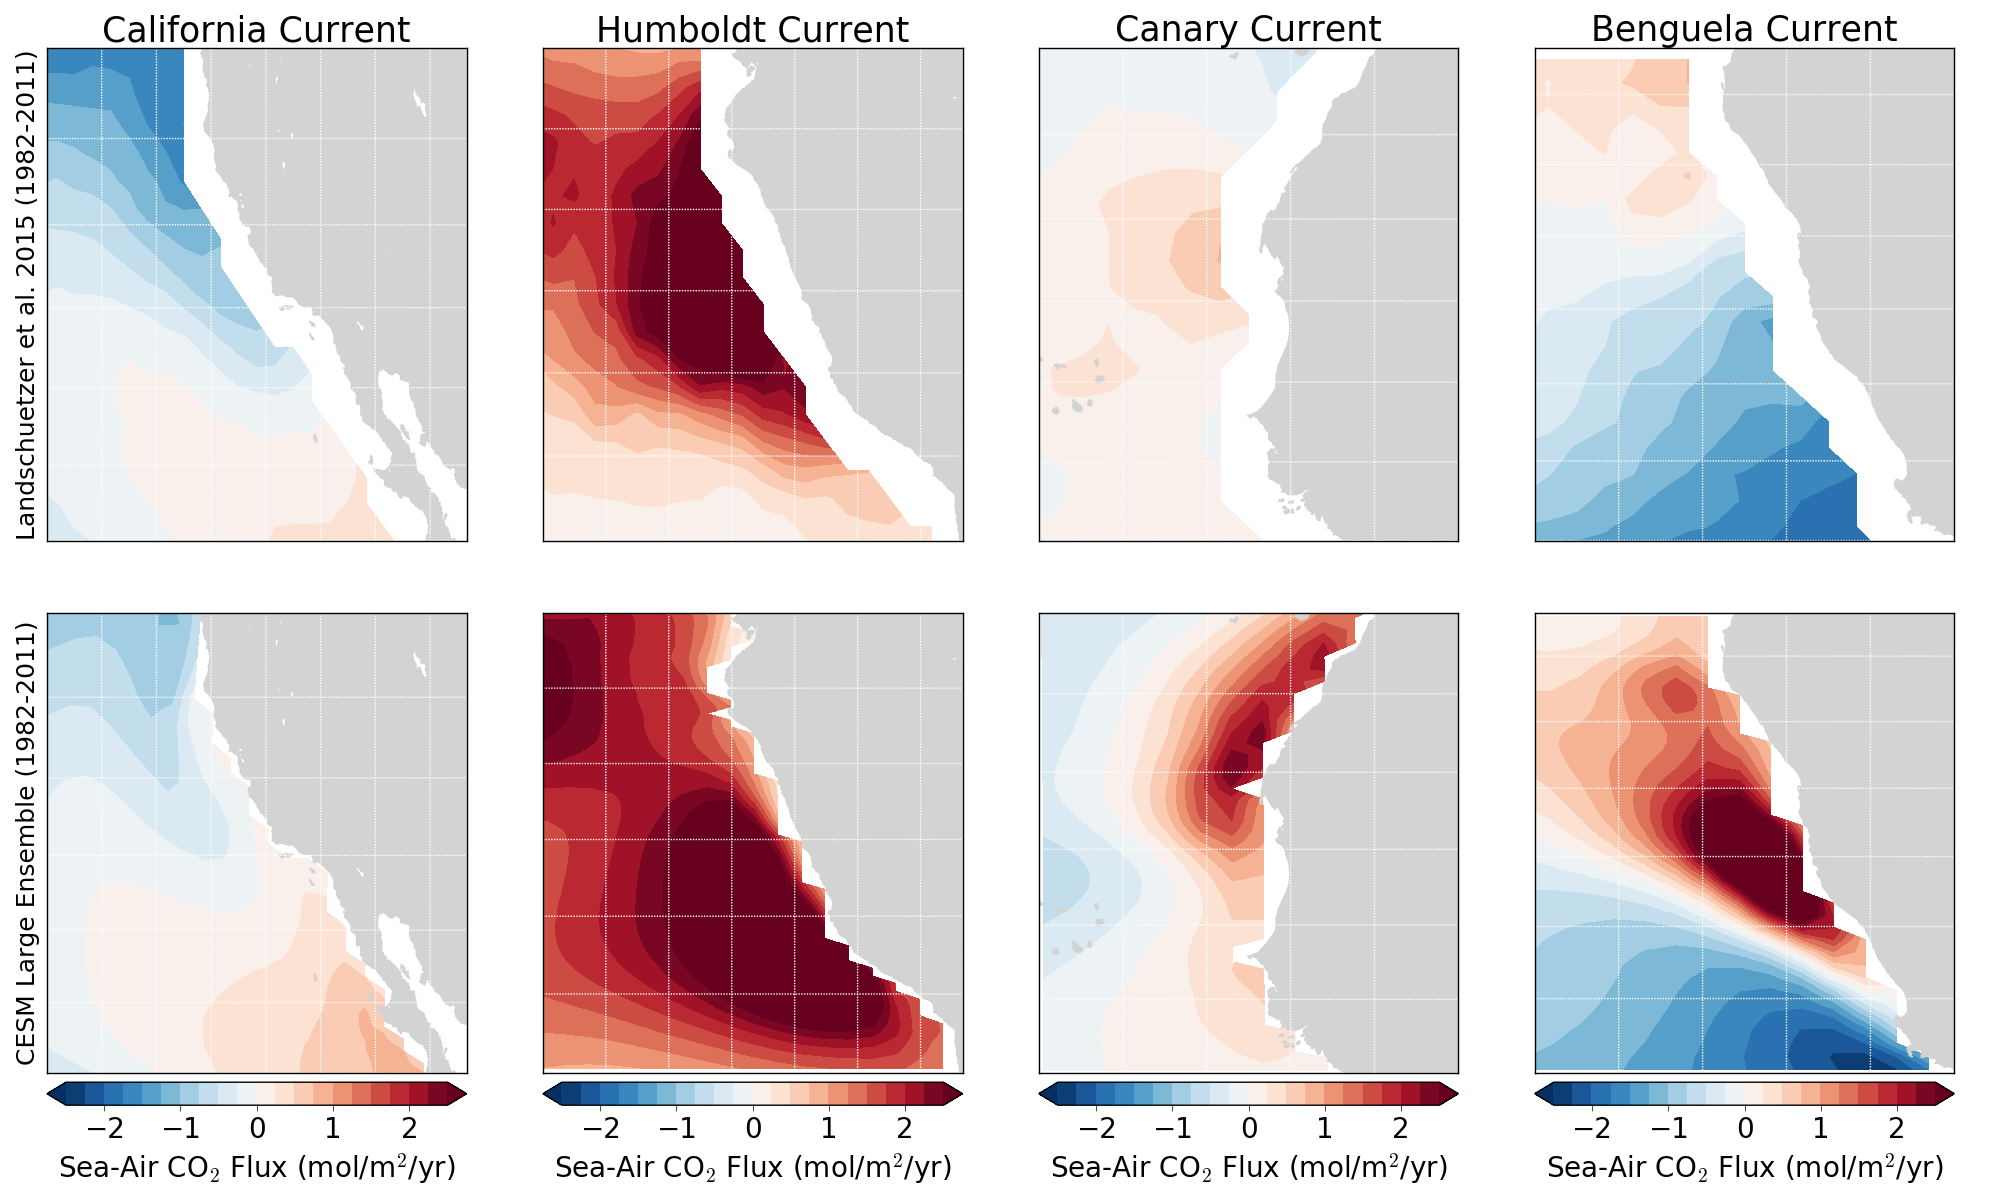
\includegraphics[width=\linewidth]{../../figs/all-systems/landschuetzer-model-climatological-comparison.png}
	\caption{Annual averages of Sea-Air CO$_{2}$ flux over 1982-2011 for the four major eastern boundary upwelling systems. The top row is observational data from \citet{Landschutzer2013}, while the bottom row is the ensemble mean from the CESM Large Ensemble. Red colors represent outgassing of CO$_{2}$, while blue colors represent uptake.}
	\label{fig:evaluation}
\end{figure}

\section{Study Sites}
For simplicity, I am using the latitudinal bounds set up by \citet{Chavez2009}, which dictates the ten degrees of most active upwelling via satellite wind stress climatology. I then constrain the offshore region to within 800km (via cell width output from the model). 
\clearpage
\begin{figure*}[!h]
    \centering
    \begin{subfigure}[b]{0.4\textwidth}
        \centering
        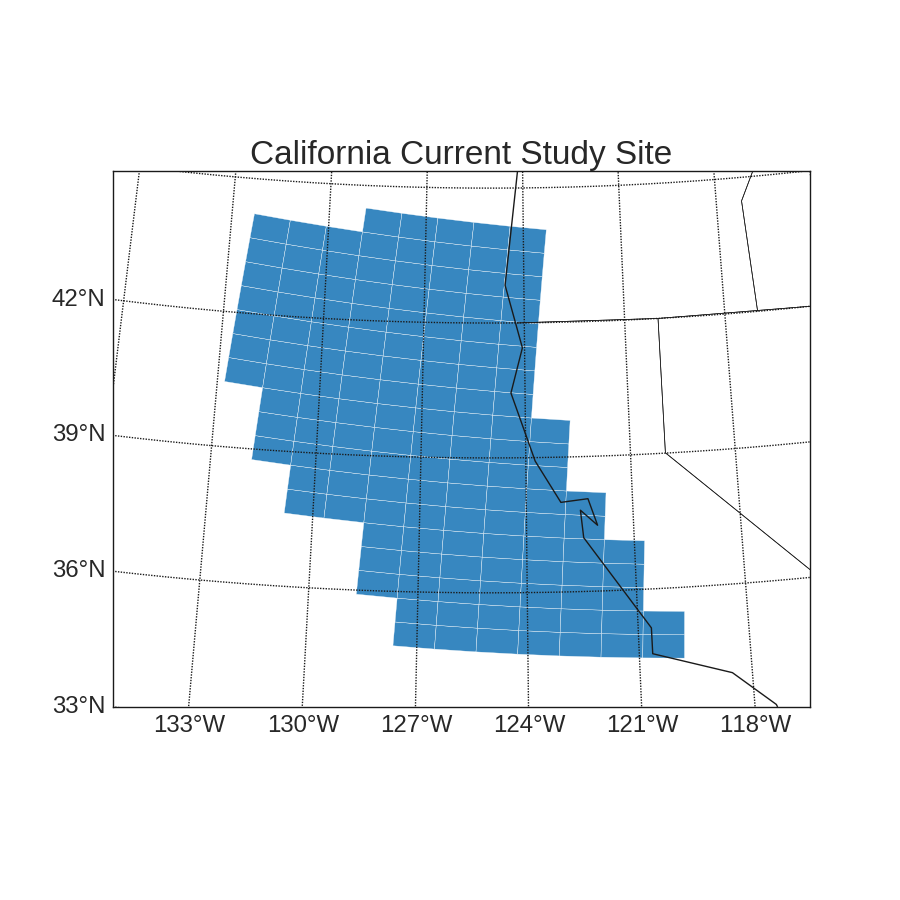
\includegraphics[width=\linewidth]{../../figs/calcs/study-site/california-current-study-site.png}
    \end{subfigure}%
    ~ 
    \begin{subfigure}[b]{0.4\textwidth}
        \centering
        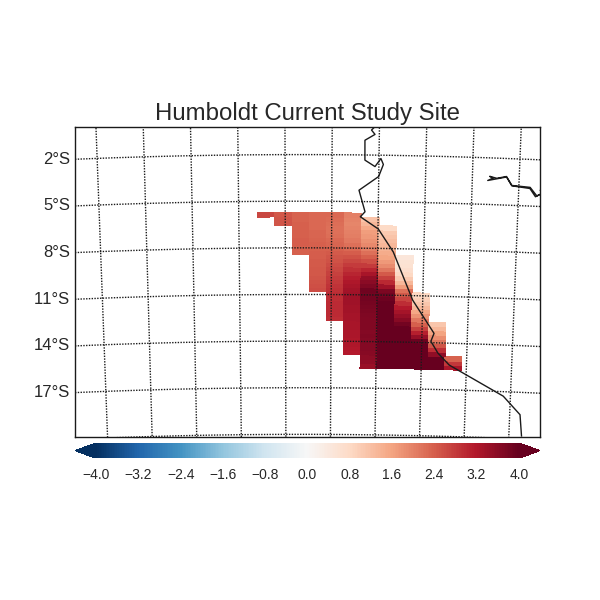
\includegraphics[width=\linewidth]{../../figs/humcs/study-site/humboldt-current-study-site.png}
    \end{subfigure} \\
    \begin{subfigure}[b]{0.4\textwidth}
        \centering
        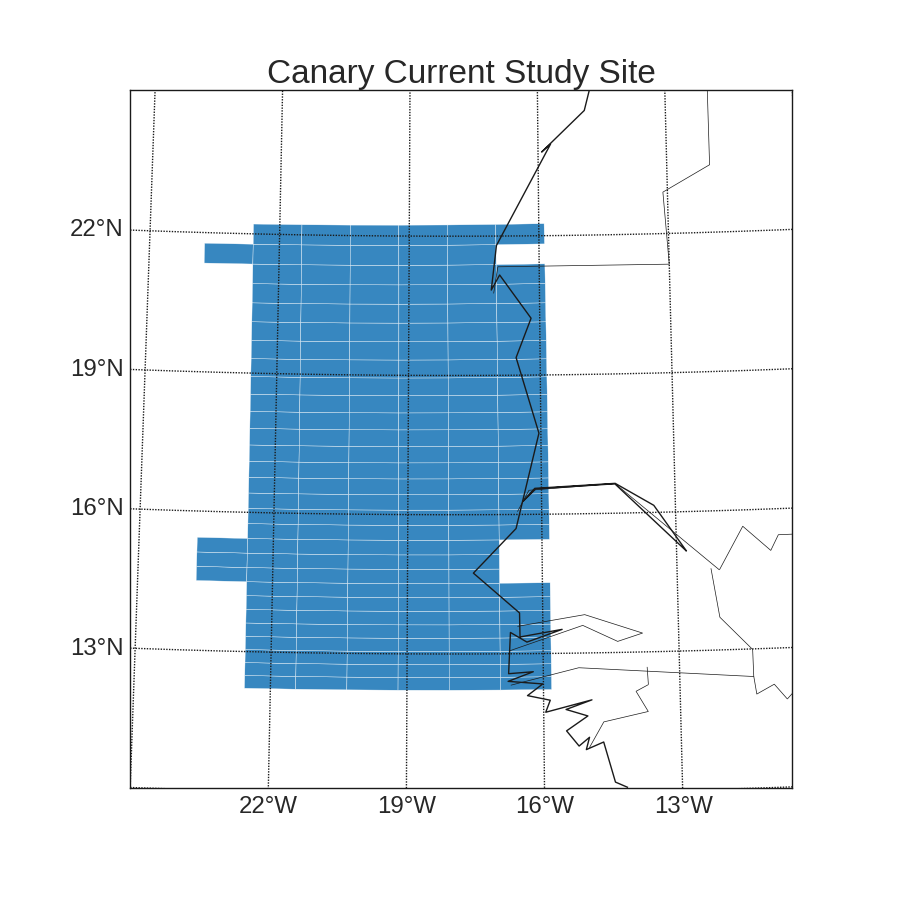
\includegraphics[width=\linewidth]{../../figs/cancs/study-site/canary-current-study-site.png}
    \end{subfigure}
    \begin{subfigure}[b]{0.4\textwidth}
        \centering
        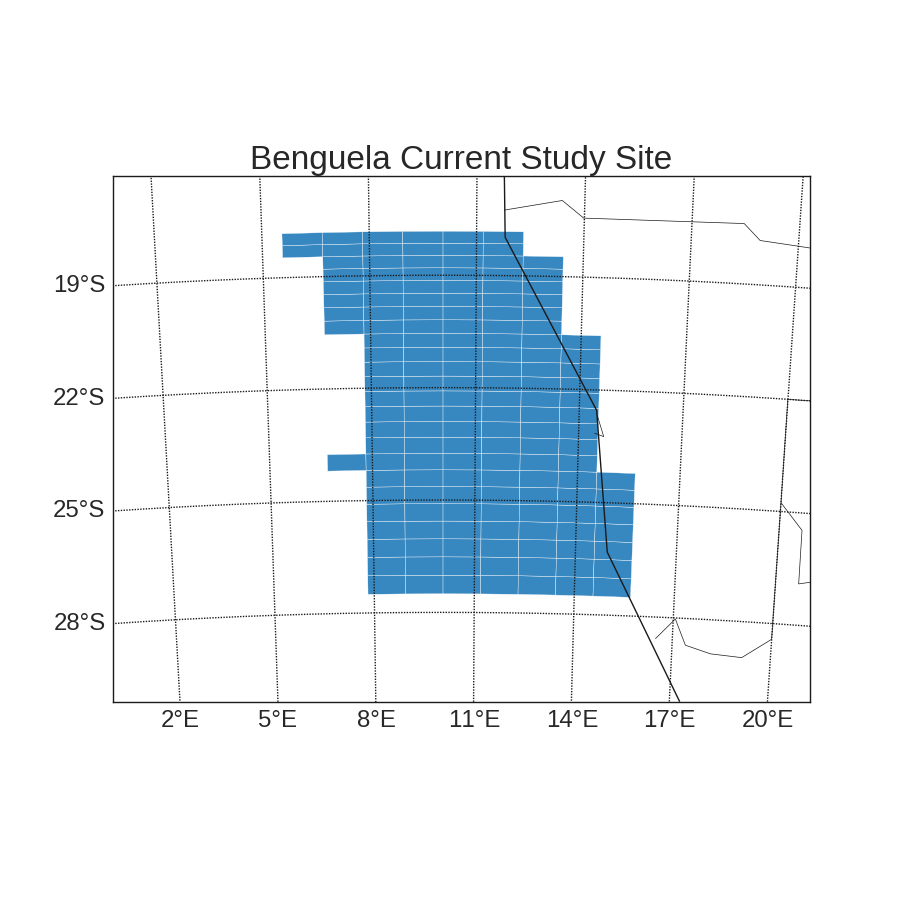
\includegraphics[width=\linewidth]{../../figs/bencs/study-site/benguela-current-study-site.png}
    \end{subfigure}
    \caption{Nearshore regions for each EBUS over which area-weighted FGCO2 is computed. The latitude is constrained by the 10 degree bounds of most active upwelling (per \citet{Chavez2009}). The longitude is constrained to 800km offshore to standardize region sizes across different latitudes.}
    \label{model:setup}
\end{figure*}

\section{General Methodology}
We use 34 CESM-LENS members, which can be treated as entirely independent time series, spanning 1920-2100 at monthly resolution. We focus, however, on the 1920-2015 period, since we are trying to understand the historical controls on FGCO2 variability (and as Adam Phillip's CVDP package covers this same period). The area-weighted mean (using TAREA) of FGCO2 is computed for each EBUS, generating a 34x1152 time series matrix. \\

First, we subtract the ensemble mean time series from each individual simulation. This de-trends the data, leaving us with 34 independent anomaly time series, which we can think of as the \it natural \rm flux of CO$_{2}$ into and out of the coastal ocean. We then load in climate index time series (Nino3.4, PDO, AMO, NAO, SAM) for the same ensemble members, and remove the linear trend from each to similarly produce anomaly time series. \\

% Add here proof that the anomaly time series are accurately describing inter-multi decadal modes of variability by performing an FFT on the raw climate indices.

We apply a 12-month (annual) rolling mean to all FGCO2 anomaly time series, as we find the raw time series to be much too noisy for meaningful correlations. See Figure~\ref{smoothed:series}, which demonstrated raw (color) time series for simulation 001 for each EBUS and the smoothed time series overlaid in black. This is defensible, as an FFT of these raw time series shows roughly red noise. \\
% Add FFT subplots.

Lastly, we regress the smoothed FGCO2 anomalies onto the four main predictors: Nino3.4, PDO, AMO, and SAM. 

\clearpage
\begin{figure*}[!h]
	\centering
	\begin{subfigure}[b]{\textwidth}
		\centering
		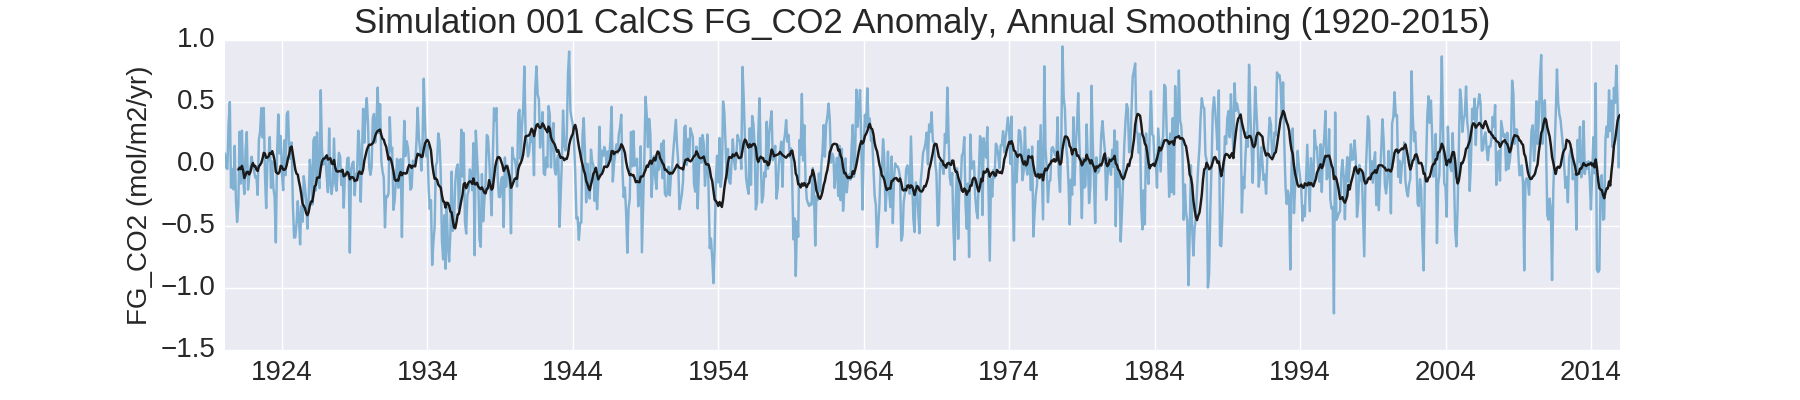
\includegraphics[width=\linewidth]{../../figs/calcs/timeseries/calcs-filtered-fgco2-series-example.png}
	\end{subfigure} \\
	\begin{subfigure}[b]{\textwidth}
		\centering
		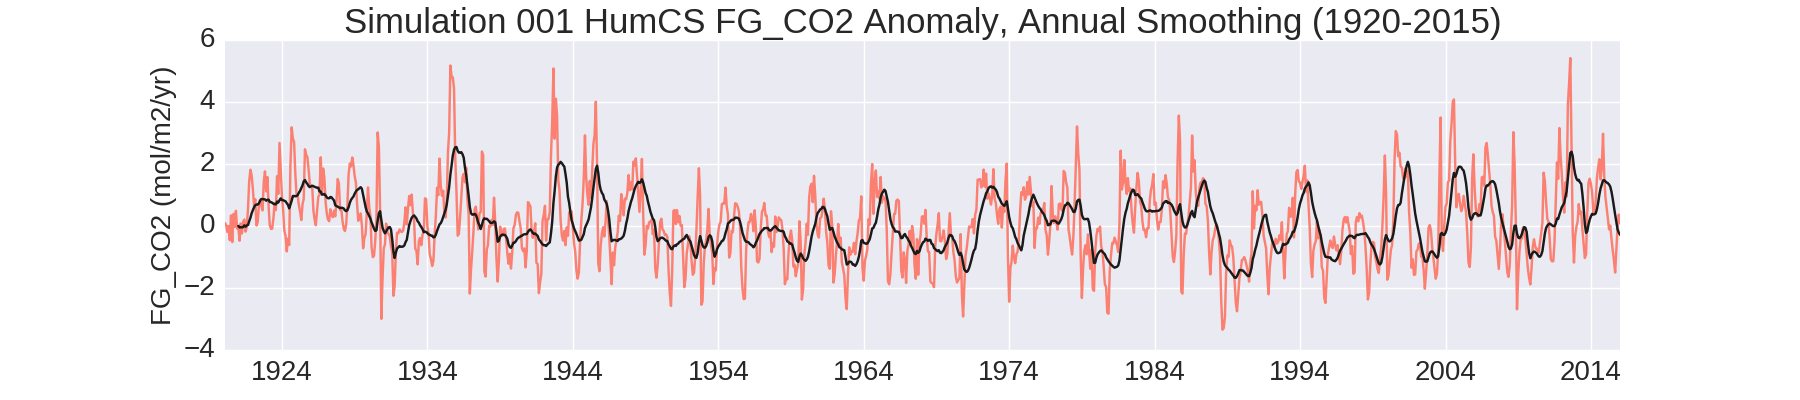
\includegraphics[width=\linewidth]{../../figs/humcs/timeseries/humcs-filtered-fgco2-series-example.png}
	\end{subfigure} \\
	\begin{subfigure}[b]{\textwidth}
		\centering
		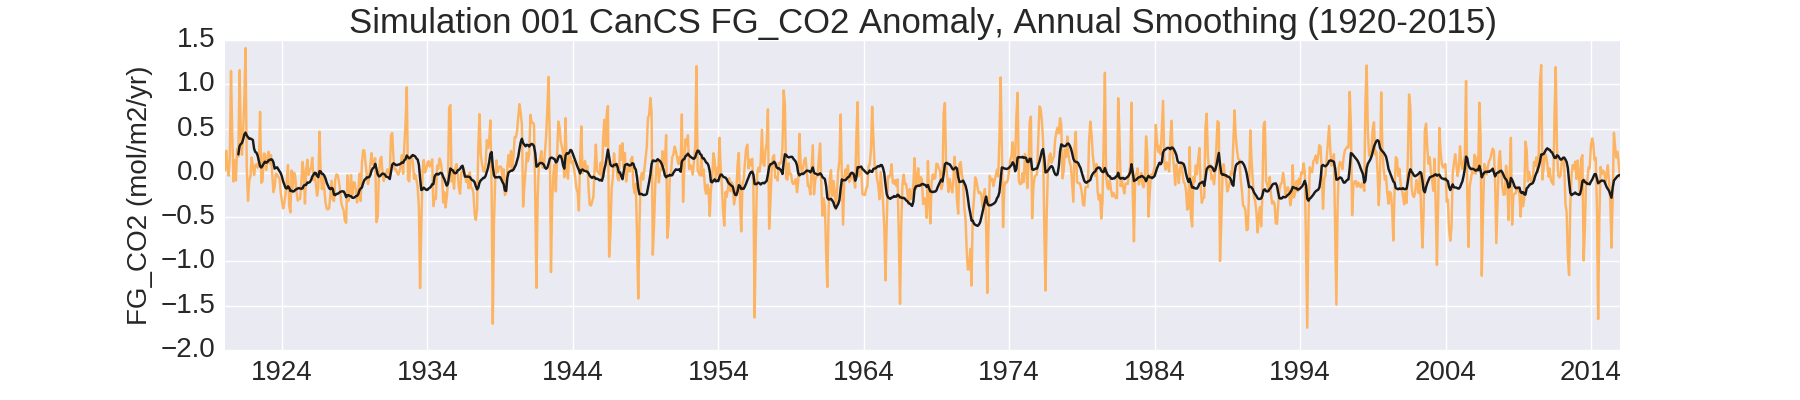
\includegraphics[width=\linewidth]{../../figs/cancs/timeseries/cancs-filtered-fgco2-series-example.png}
	\end{subfigure} \\
	\begin{subfigure}[b]{\textwidth}
		\centering
		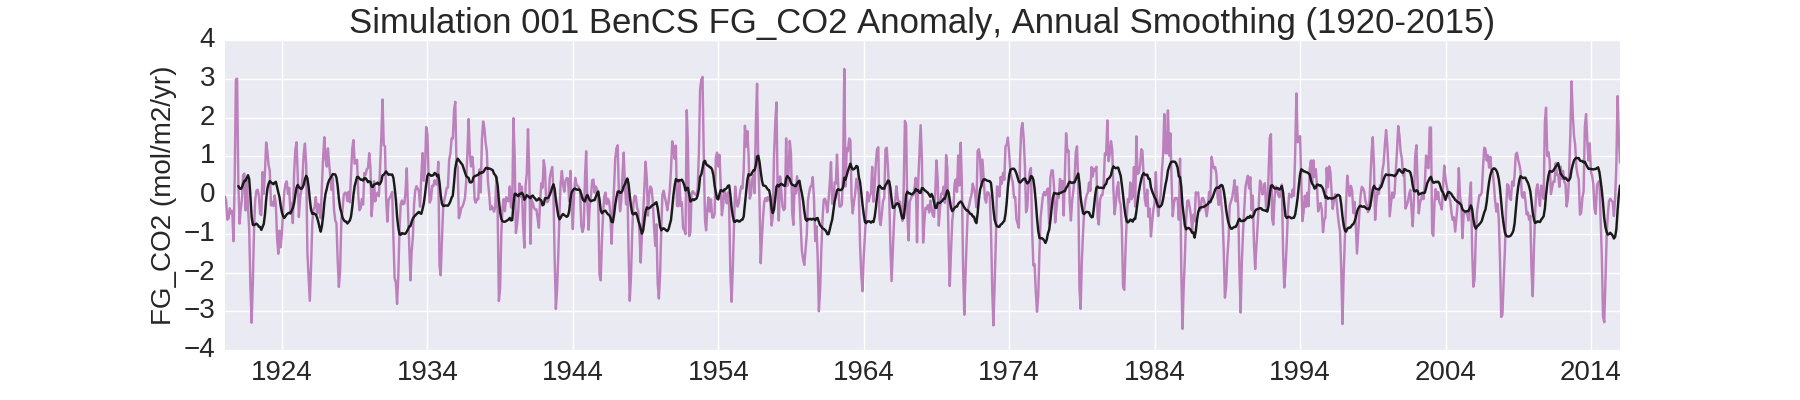
\includegraphics[width=\linewidth]{../../figs/bencs/timeseries/bencs-filtered-fgco2-series-example.png}
	\end{subfigure}
	\caption{FGCO2 anomalies for arbitrary simulation 001 in color with their annual smoothing counterpart overlaid in black.}
	\label{smoothed:series}
\end{figure*}

\section{Climate Correlations}
I have split the analysis into the two major ocean basins that house our four EBUS. This is because (1) it eases the viewing and interpretation of statistical tests, and (2) we might glean some similarities and differences between the two basins. 

\subsection{Pacific Sector}
Figure~\ref{fig:pacific-histograms} displays the results of using four climate indices (Nino3.4, PDO, AMO, and SAM) as predictors for CalCS and HumCS natural CO$_{2}$ fluxes over the 1920-2015 period. We find that ENSO and PDO have the largest influence on natural CO$_{2}$ flux variability, and have inverse impacts on the two systems. \\

During an El Ni\~no event, more CO$_{2}$ fluxes out of the CalCS, while more CO$_{2}$ is taken up by the HumCS. Perhaps this illuminates the dependency of CalCS FGCO2 on SST variability, which would alter the solubility of pCO$_{2}$; during a warm event, low pCO$_{2}$ solubility would force carbon out of the CalCS. On the other hand, SSTs might be more stable in the more tropical HumCS, so FGCO2 variability could be more dependent on DIC delivery from depth. During El Ni\~no events, upwelling of high-DIC water would be suppressed, leading to an influx of carbon. These ideas can be tested by using Takahashi formulae to separate temperature-dependent pCO$_{2}$ effects from non-temperature-dependent effects. These arguments might also hold for the PDO, since it has a large impact on Pacific Ocean SST patterns. Raw values for the regression slope, r-value, and r$^{2}$ can be found in Table~\ref{tab:enso-pacific} (Nino3.4) and Table~\ref{tab:pdo-pacific} (PDO). \\

An interesting result is that AMO has a small, but discernible correlation with CalCS CO$_{2}$ flux, but hovers around an r-value of zero for the HumCS. Perhaps atmospheric teleconnections between the North Atlantic and North Pacific play a role here.
 
\begin{figure}[!h]
	\centering
	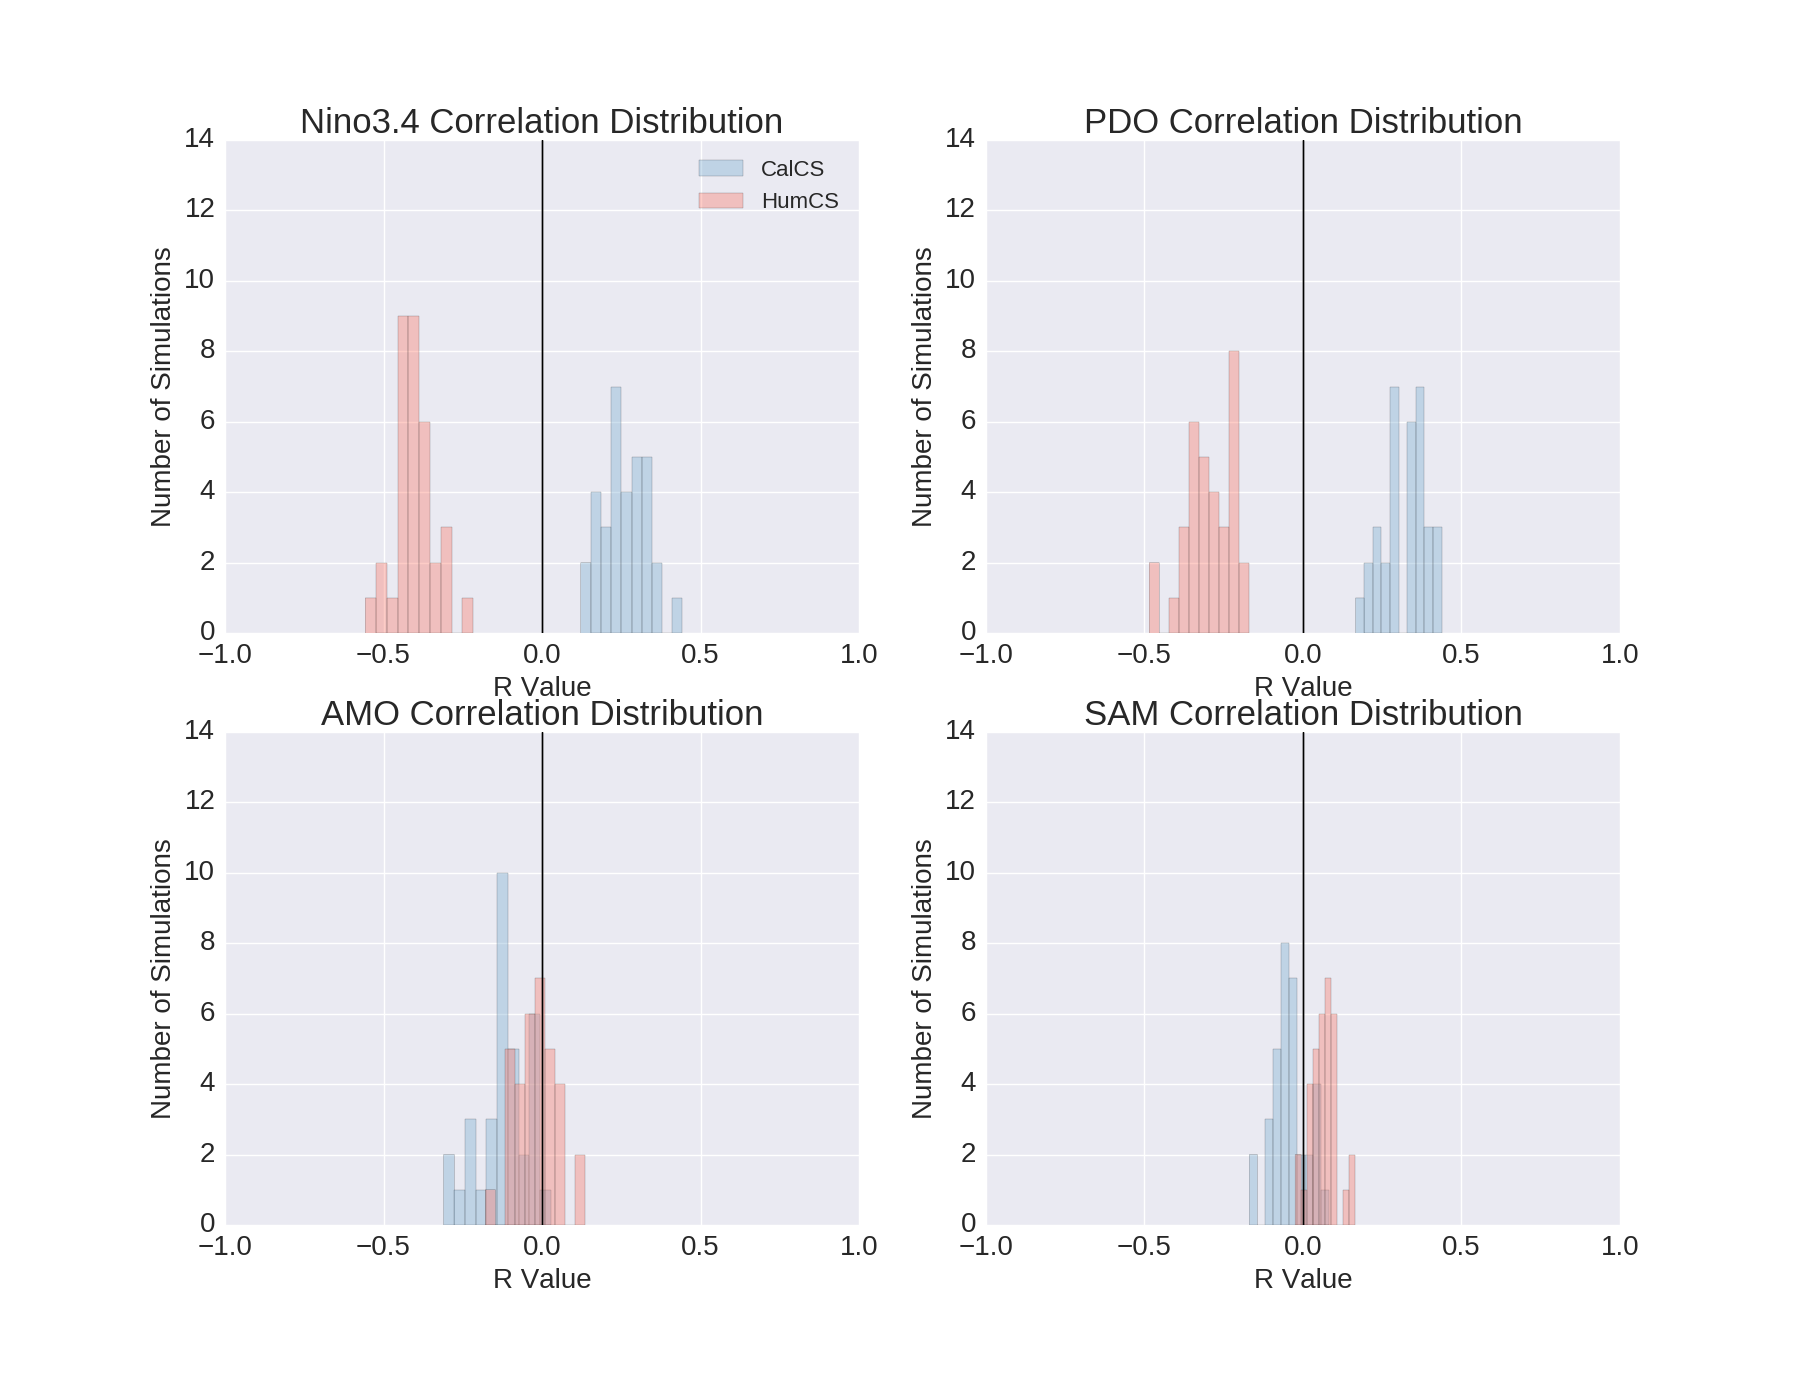
\includegraphics[width=\linewidth]{../../figs/pacific/pacific-EBU-correlation-distributions.png}
	\caption{R values for annually smoothed FGCO2 anomalies in the CalCS and HumCS compared to four major climate indices. Correlations with $p$ $>$ 0.05 were not included.}
	\label{fig:pacific-histograms}
\end{figure}

\newpage
\begin{table}[!h]
	\centering
	\caption{Results for regressing FGCO2 anomalies onto Nino3.4 time series for the two Pacific upwelling systems. Results with $p$ $>$ 0.05 are excluded.}
\begin{tabular}{c c c c | c c c}
	& \multicolumn{3}{c}{CalCS} & \multicolumn{3}{c}{HumCS} \\
	\cmidrule{2-4}\cmidrule{5-7}
	\textbf{Simulation} &  \textbf{Slope}$^{a}$  &  \textbf{R} &  \textbf{R$^{2}$} &  \textbf{Slope}$^{a}$  &  \textbf{R} &  \textbf{R$^{2}$}  \\
	\midrule
	001 &   0.04 &     0.30 &       0.09 &  -0.20 &    -0.29 &       0.08 \\
	002 &   0.06 &     0.33 &       0.11 &  -0.31 &    -0.35 &       0.12 \\
	009 &   0.03 &     0.18 &       0.03 &  -0.24 &    -0.31 &       0.10 \\
	010 &   0.04 &     0.22 &       0.05 &  -0.33 &    -0.44 &       0.19 \\
	011 &    - &      - &                    -  &  -0.28 &    -0.39 &       0.15 \\
	012 &   0.05 &     0.28 &       0.08 &  -0.31 &    -0.43 &       0.19 \\
	013 &   0.06 &     0.33 &       0.11 &  -0.33 &    -0.42 &       0.17 \\
	014 &   0.05 &     0.35 &       0.12 &  -0.30 &    -0.44 &       0.19 \\
	015 &   0.05 &     0.29 &       0.08 &  -0.34 &    -0.44 &       0.20 \\
	016 &   0.04 &     0.22 &       0.05 &  -0.32 &    -0.38 &       0.14 \\
	017 &   0.04 &     0.27 &       0.07 &  -0.26 &    -0.45 &       0.20 \\
	018 &   0.05 &     0.29 &       0.08 &  -0.33 &    -0.40 &       0.16 \\
	019 &   0.04 &     0.21 &       0.04 &  -0.35 &    -0.43 &       0.19 \\
	020 &   0.05 &     0.30 &       0.09 &  -0.22 &    -0.36 &       0.13 \\
	021 &   0.03 &     0.18 &       0.03 &  -0.28 &    -0.36 &       0.13 \\
	022 &   0.04 &     0.24 &       0.06 &  -0.37 &    -0.46 &       0.22 \\
	023 &   0.03 &     0.22 &       0.05 &  -0.31 &    -0.37 &       0.14 \\
	024 &   0.06 &     0.33 &       0.11 &  -0.33 &    -0.44 &       0.19 \\
	025 &   0.05 &     0.34 &       0.12 &  -0.29 &    -0.40 &       0.16 \\
	026 &   0.04 &     0.25 &       0.06 &  -0.32 &    -0.39 &       0.15 \\
	027 &   0.04 &     0.28 &       0.08 &  -0.22 &    -0.30 &       0.09 \\
	028 &   0.03 &     0.17 &       0.03 &  -0.26 &    -0.38 &       0.15 \\
	029 &   0.05 &     0.33 &       0.11 &  -0.39 &    -0.46 &       0.21 \\
	030 &   0.03 &     0.19 &       0.04 &  -0.30 &    -0.42 &       0.17 \\
	031 &   0.04 &     0.24 &       0.06 &  -0.34 &    -0.42 &       0.18 \\
	032 &   0.04 &     0.20 &       0.04 &  -0.39 &    -0.51 &       0.26 \\
	033 &   0.02 &     0.14 &       0.02 &  -0.14 &    -0.22 &       0.05 \\
	034 &   0.06 &     0.31 &       0.10 &  -0.25 &    -0.32 &       0.10 \\
	035 &   0.03 &     0.17 &       0.03 &  -0.31 &    -0.42 &       0.18 \\
	101 &   0.07 &     0.44 &       0.20 &  -0.28 &    -0.41 &       0.17 \\
	102 &   0.04 &     0.26 &       0.07 &  -0.24 &    -0.40 &       0.16 \\
	103 &   0.04 &     0.22 &       0.05 &  -0.29 &    -0.40 &       0.16 \\
	104 &   0.05 &     0.35 &       0.12 &  -0.41 &    -0.56 &       0.31 \\
	105 &   0.02 &     0.12 &       0.01 &  -0.45 &    -0.49 &       0.24 \\
	\bottomrule
	\textbf{Mean} & 0.04 & 0.26 & 0.07 & -0.30 & -0.40 & 0.17 \\
	\textbf{Std} & 0.01 & 0.07 & 0.04 & 0.06 & 0.06 & 0.05
\end{tabular}
\begin{tablenotes}
	\centering
	\item $^{a}$ mol/m$^{2}$/yr/degC
\end{tablenotes}
\label{tab:enso-pacific}
\end{table}

\newpage
\begin{table}[!h]
	\centering
	\caption{Results for regressing FGCO2 anomalies onto PDO time series for the two Pacific upwelling systems. Results with $p$ $>$ 0.05 are excluded.}
	\begin{tabular}{c c c c | c c c}
		& \multicolumn{3}{c}{CalCS} & \multicolumn{3}{c}{HumCS} \\
		\cmidrule{2-4}\cmidrule{5-7}
		\textbf{Simulation} &  \textbf{Slope}$^{a}$  &  \textbf{R} &  \textbf{R$^{2}$} &  \textbf{Slope}$^{a}$  &  \textbf{R} &  \textbf{R$^{2}$}  \\
		\midrule
		001 &   0.06 &     0.38 &       0.14 &  -0.23 &    -0.28 &       0.08 \\
		002 &   0.06 &     0.35 &       0.12 &  -0.20 &    -0.24 &       0.06 \\
		009 &   0.06 &     0.36 &       0.13 &  -0.17 &    -0.22 &       0.05 \\
		010 &   0.06 &     0.35 &       0.12 &  -0.27 &    -0.36 &       0.13 \\
		011 &   0.03 &     0.17 &       0.03 &  -0.29 &    -0.38 &       0.14 \\
		012 &   0.07 &     0.38 &       0.15 &  -0.20 &    -0.25 &       0.06 \\
		013 &   0.04 &     0.25 &       0.06 &  -0.22 &    -0.30 &       0.09 \\
		014 &   0.06 &     0.34 &       0.11 &  -0.25 &    -0.30 &       0.09 \\
		015 &   0.05 &     0.29 &       0.09 &  -0.17 &    -0.23 &       0.05 \\
		016 &   0.05 &     0.28 &       0.08 &  -0.18 &    -0.22 &       0.05 \\
		017 &   0.06 &     0.37 &       0.14 &  -0.23 &    -0.34 &       0.11 \\
		018 &   0.05 &     0.28 &       0.08 &  -0.14 &    -0.17 &       0.03 \\
		019 &   0.07 &     0.36 &       0.13 &  -0.26 &    -0.32 &       0.10 \\
		020 &   0.06 &     0.37 &       0.14 &  -0.26 &    -0.38 &       0.15 \\
		021 &   0.04 &     0.26 &       0.07 &  -0.27 &    -0.35 &       0.12 \\
		022 &   0.07 &     0.40 &       0.16 &  -0.29 &    -0.35 &       0.12 \\
		023 &   0.05 &     0.37 &       0.14 &  -0.16 &    -0.19 &       0.04 \\
		024 &   0.08 &     0.44 &       0.19 &  -0.26 &    -0.34 &       0.12 \\
		025 &   0.07 &     0.41 &       0.17 &  -0.25 &    -0.30 &       0.09 \\
		026 &   0.05 &     0.33 &       0.11 &  -0.17 &    -0.21 &       0.04 \\
		027 &   0.03 &     0.19 &       0.04 &  -0.24 &    -0.29 &       0.08 \\
		028 &   0.07 &     0.43 &       0.19 &  -0.20 &    -0.31 &       0.09 \\
		029 &   0.03 &     0.22 &       0.05 &  -0.26 &    -0.27 &       0.07 \\
		030 &   0.05 &     0.27 &       0.07 &  -0.17 &    -0.23 &       0.05 \\
		031 &   0.05 &     0.30 &       0.09 &  -0.24 &    -0.29 &       0.08 \\
		032 &   0.05 &     0.29 &       0.09 &  -0.35 &    -0.48 &       0.23 \\
		033 &   0.05 &     0.34 &       0.11 &  -0.15 &    -0.21 &       0.04 \\
		034 &   0.04 &     0.23 &       0.05 &  -0.16 &    -0.21 &       0.04 \\
		035 &   0.04 &     0.23 &       0.05 &  -0.17 &    -0.23 &       0.05 \\
		101 &   0.05 &     0.29 &       0.08 &  -0.27 &    -0.35 &       0.12 \\
		102 &   0.07 &     0.39 &       0.15 &  -0.28 &    -0.39 &       0.15 \\
		103 &   0.06 &     0.34 &       0.11 &  -0.25 &    -0.35 &       0.12 \\
		104 &   0.06 &     0.39 &       0.15 &  -0.42 &    -0.48 &       0.23 \\
		105 &   0.05 &     0.30 &       0.09 &  -0.24 &    -0.26 &       0.07 \\
		\bottomrule
		\textbf{Mean} & 0.05 & 0.32 & 0.11 & -0.23 & -0.30 & 0.09 \\
		\textbf{Std} & 0.01 & 0.07 & 0.04 & 0.06 & 0.08 & 0.05
	\end{tabular}
	\begin{tablenotes}
		\centering
		\item $^{a}$ mol/m$^{2}$/yr/degC
	\end{tablenotes}
	\label{tab:pdo-pacific}
\end{table}
\clearpage
\subsection{Atlantic Sector}
Figure~\ref{fig:atlantic-histograms} displays distributions of correlation tests between FGCO2 anomalies in the two Atlantic Ocean EBUS (Canary and Benguela) and the same four climate indices. At first glance, the results are much weaker than that of the Pacific systems. I find it surprising that the SAM has virtually no impact on the BenCS, when it is the only EBUS that interfaces directly with the Southern Ocean. \\

Interestingly, CanCS gas flux has a reasonable relationship with ENSO and the PDO. As much as 15\% of FGCO2 variability in the CanCS can be explained by ENSO in some simulations (Table~\ref{tab:enso-atlantic}). We find a similar situation with regards to the PDO (Table~\ref{tab:pdo-atlantic}). There is a slight relationship between FGCO2 anomalies in the CanCS and the AMO, but it isn't even as strong as the correlation with ENSO and PDO. Overall, the BenCS is not well-explained by any major climate index.

\begin{figure}[!h]
	\centering
	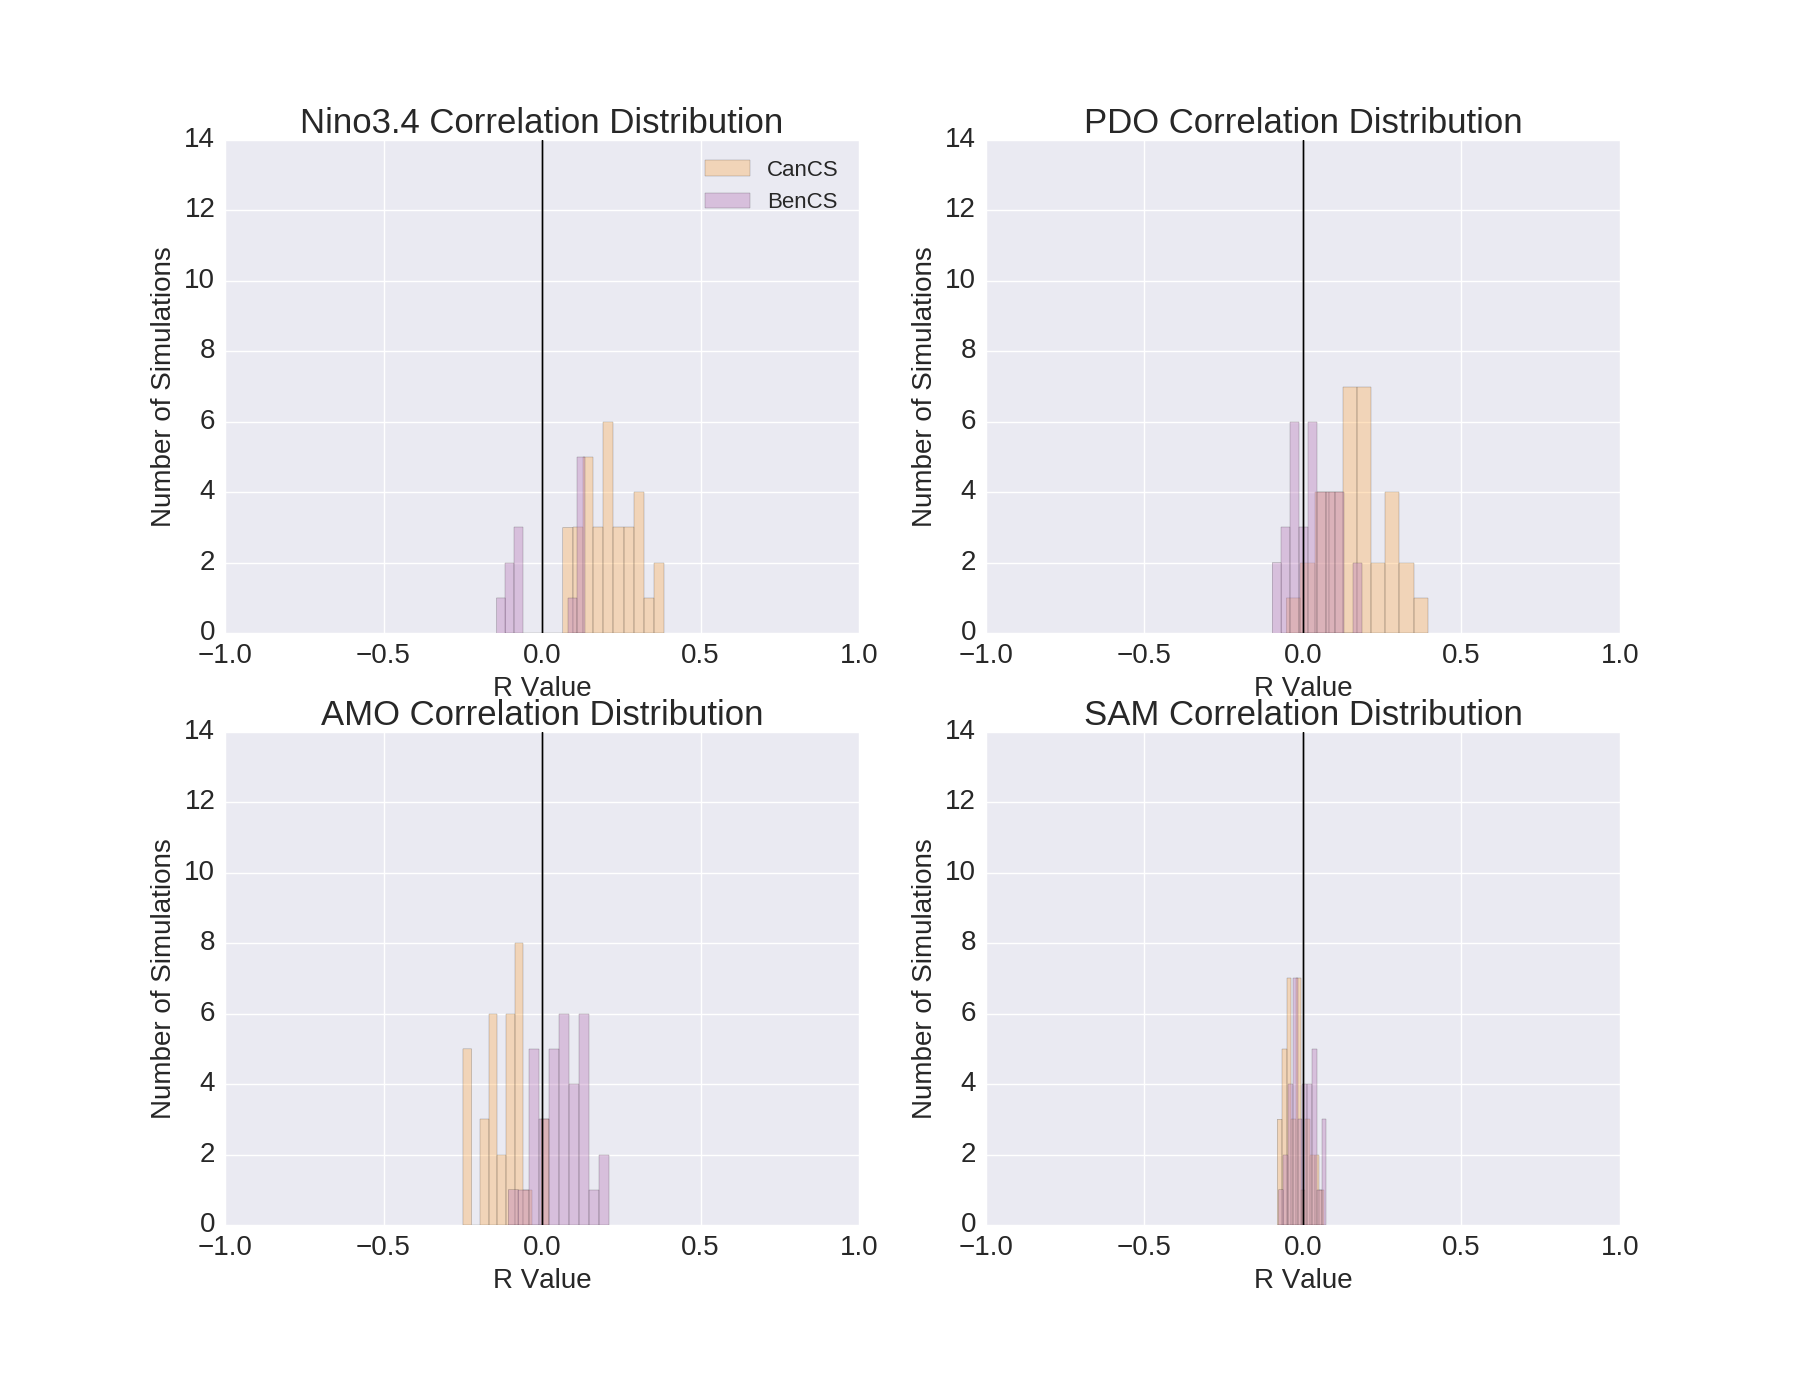
\includegraphics[width=\linewidth]{../../figs/atlantic/atlantic-EBU-correlation-distributions.png}
	\caption{R values for annually smoothed FGCO2 anomalies in the CalCS and HumCS compared to four major climate indices. Correlations with $p$ $>$ 0.05 were not included.}
	\label{fig:atlantic-histograms}
\end{figure}

\newpage
\begin{table}[!h]
	\centering
	\caption{Results for regressing FGCO2 anomalies onto ENSO time series for the two Atlantic upwelling systems. Results with $p$ $>$ 0.05 are excluded.}
	\begin{tabular}{c c c c | c c c}
		& \multicolumn{3}{c}{CanCS} & \multicolumn{3}{c}{BenCS} \\
		\cmidrule{2-4}\cmidrule{5-7}
		\textbf{Simulation} &  \textbf{Slope}$^{a}$  &  \textbf{R} &  \textbf{R$^{2}$} &  \textbf{Slope}$^{a}$  &  \textbf{R} &  \textbf{R$^{2}$}  \\
		\midrule
		001 &   0.04 &     0.28 &       0.08 &    - &      - &        - \\
		002 &   0.06 &     0.31 &       0.10 &    - &      - &        - \\
		009 &   0.03 &     0.18 &       0.03 &    - &      - &        - \\
		010 &   0.05 &     0.29 &       0.08 &    - &      - &        - \\
		011 &   0.04 &     0.25 &       0.06 &   0.05 &     0.13 &       0.02 \\
		012 &   0.04 &     0.28 &       0.08 &  -0.05 &    -0.11 &       0.01 \\
		013 &   0.04 &     0.22 &       0.05 &    - &      - &        - \\
		014 &   0.05 &     0.34 &       0.12 &    - &      - &        - \\
		015 &   0.03 &     0.16 &       0.03 &    - &      - &        - \\
		016 &   0.02 &     0.10 &       0.01 &    - &      - &        - \\
		017 &   0.05 &     0.38 &       0.15 &    - &      - &        - \\
		018 &   0.03 &     0.17 &       0.03 &  -0.07 &    -0.14 &       0.02 \\
		019 &   0.02 &     0.11 &       0.01 &   0.04 &     0.09 &       0.01 \\
		020 &   0.05 &     0.32 &       0.10 &    - &      - &        - \\
		021 &   0.02 &     0.12 &       0.01 &    - &      - &        - \\
		022 &   0.02 &     0.15 &       0.02 &   0.06 &     0.12 &       0.01 \\
		023 &   0.04 &     0.22 &       0.05 &    - &      - &        - \\
		024 &   0.04 &     0.25 &       0.06 &   0.06 &     0.13 &       0.02 \\
		025 &   0.01 &     0.08 &       0.01 &    - &      - &        - \\
		026 &   0.05 &     0.27 &       0.07 &  -0.04 &    -0.09 &       0.01 \\
		027 &   0.03 &     0.20 &       0.04 &   0.07 &     0.14 &       0.02 \\
		028 &   0.01 &     0.07 &       0.00 &   0.06 &     0.13 &       0.02 \\
		029 &   0.05 &     0.31 &       0.10 &    - &      - &        - \\
		031 &   0.02 &     0.15 &       0.02 &    - &      - &        - \\
		032 &   0.03 &     0.15 &       0.02 &    - &      - &        - \\
		033 &   0.03 &     0.21 &       0.04 &  -0.03 &    -0.08 &       0.01 \\
		034 &   0.03 &     0.17 &       0.03 &  -0.05 &    -0.11 &       0.01 \\
		035 &   0.01 &     0.07 &       0.00 &  -0.03 &    -0.07 &       0.00 \\
		101 &   0.03 &     0.22 &       0.05 &    - &      - &        - \\
		102 &   0.03 &     0.19 &       0.04 &    - &      - &        - \\
		103 &   0.07 &     0.39 &       0.15 &    - &      - &        - \\
		104 &   0.03 &     0.23 &       0.05 &    - &      - &        - \\
		105 &   0.02 &     0.13 &       0.02 &    - &      - &        - \\
		\bottomrule
		\textbf{Mean} & 0.03 & 0.21 & 0.05 & 0.01 & 0.01 & 0.01 \\
		\textbf{Std} & 0.01 & 0.09 & 0.04 & 0.05 & 0.11 & 0.01
	\end{tabular}
	\begin{tablenotes}
		\centering
		\item $^{a}$ mol/m$^{2}$/yr/degC
	\end{tablenotes}
	\label{tab:enso-atlantic}
\end{table}

\newpage
\begin{table}[!h]
	\centering
	\caption{Results for regressing FGCO2 anomalies onto PDO time series for the two Atlantic upwelling systems. Results with $p$ $>$ 0.05 are excluded.}
	\begin{tabular}{c c c c | c c c}
		& \multicolumn{3}{c}{CanCS} & \multicolumn{3}{c}{BenCS} \\
		\cmidrule{2-4}\cmidrule{5-7}
		\textbf{Simulation} &  \textbf{Slope}$^{a}$  &  \textbf{R} &  \textbf{R$^{2}$} &  \textbf{Slope}$^{a}$  &  \textbf{R} &  \textbf{R$^{2}$}  \\
		\midrule
		001 &   0.05 &     0.30 &       0.09 &  -0.01 &    -0.02 &       0.00 \\
		002 &   0.07 &     0.39 &       0.15 &  -0.00 &    -0.00 &       0.00 \\
		009 &   0.02 &     0.11 &       0.01 &  -0.03 &    -0.05 &       0.00 \\
		010 &   0.05 &     0.28 &       0.08 &  -0.01 &    -0.01 &       0.00 \\
		011 &   0.03 &     0.17 &       0.03 &   0.01 &     0.02 &       0.00 \\
		012 &   0.02 &     0.11 &       0.01 &   0.02 &     0.04 &       0.00 \\
		013 &   0.03 &     0.21 &       0.04 &   0.02 &     0.03 &       0.00 \\
		014 &   0.05 &     0.27 &       0.07 &  -0.02 &    -0.04 &       0.00 \\
		015 &   0.02 &     0.11 &       0.01 &   0.03 &     0.07 &       0.01 \\
		016 &   0.02 &     0.14 &       0.02 &   0.04 &     0.07 &       0.01 \\
		017 &   0.04 &     0.22 &       0.05 &  -0.02 &    -0.05 &       0.00 \\
		018 &   0.01 &     0.08 &       0.01 &  -0.01 &    -0.01 &       0.00 \\
		019 &   0.01 &     0.06 &       0.00 &   0.09 &     0.19 &       0.03 \\
		020 &   0.02 &     0.13 &       0.02 &  -0.00 &    -0.01 &       0.00 \\
		021 &   0.01 &     0.06 &       0.00 &   0.06 &     0.13 &       0.02 \\
		022 &   0.03 &     0.16 &       0.03 &   0.09 &     0.18 &       0.03 \\
		023 &  -0.01 &    -0.05 &       0.00 &  -0.01 &    -0.02 &       0.00 \\
		024 &   0.02 &     0.11 &       0.01 &   0.04 &     0.08 &       0.01 \\
		025 &   0.03 &     0.17 &       0.03 &  -0.04 &    -0.08 &       0.01 \\
		026 &   0.02 &     0.13 &       0.02 &   0.02 &     0.05 &       0.00 \\
		027 &   0.03 &     0.19 &       0.03 &   0.06 &     0.10 &       0.01 \\
		028 &   0.02 &     0.13 &       0.02 &   0.05 &     0.11 &       0.01 \\
		029 &   0.06 &     0.33 &       0.11 &   0.06 &     0.12 &       0.01 \\
		030 &   0.01 &     0.05 &       0.00 &   0.05 &     0.10 &       0.01 \\
		031 &   0.00 &     0.02 &       0.00 &  -0.01 &    -0.02 &       0.00 \\
		032 &   0.03 &     0.20 &       0.04 &  -0.03 &    -0.06 &       0.00 \\
		033 &   0.03 &     0.22 &       0.05 &   0.01 &     0.02 &       0.00 \\
		034 &   0.03 &     0.14 &       0.02 &  -0.05 &    -0.10 &       0.01 \\
		035 &   0.02 &     0.15 &       0.02 &   0.02 &     0.04 &       0.00 \\
		101 &   0.01 &     0.04 &       0.00 &   0.03 &     0.05 &       0.00 \\
		102 &   0.03 &     0.19 &       0.03 &   0.00 &     0.01 &       0.00 \\
		103 &   0.05 &     0.31 &       0.09 &   0.06 &     0.12 &       0.01 \\
		104 &   0.04 &     0.27 &       0.07 &   0.02 &     0.03 &       0.00 \\
		105 &   0.03 &     0.19 &       0.04 &   0.02 &     0.05 &       0.00 \\
		\bottomrule
		\textbf{Mean} & 0.03 & 0.16 & 0.04 & 0.02 & 0.03 & 0.01 \\
		\textbf{Std} & 0.02 & 0.09 & 0.04 & 0.03 & 0.07 & 0.01
	\end{tabular}
	\begin{tablenotes}
		\centering
		\item $^{a}$ mol/m$^{2}$/yr/degC
	\end{tablenotes}
	\label{tab:pdo-atlantic}
\end{table}

\section{Cross Correlation}
Perhaps we are underestimating the strength of relationship between some climate indices and EBU CO$_{2}$ flux, as we are not lagging/leading the correlations properly. Due to the physical mechanisms behind ENSO, there might be a sort of lag between a strong El Ni\~no and an anomalous gas flux. Since we are trying to understand controls on CO$_{2}$ flux variability, it probably only makes sense to look at situations where the climate index leads the gas flux anomalies. \\

Figure~\ref{fig:CalCS-ENSO-Cross} shows little consistency in enhanced correlations at any lead/lag. I would argue that there is little sense in correlating anything but lag zero in the case of CalCS and Nino3.4. However, turning our attention to the HumCS, we find a strong case to compute a lag correlation for ENSO, rather than a standard lag zero correlation (Figure~\ref{fig:HumCS-ENSO-Cross}). In 100\% of the simulations, the correlation is stronger when leading FGCO2 anomalies by 4-5 months with the Nino3.4 index. \\

Table~\ref{tab:HumCS-ENSO-5lag} displays the results of a regression analysis between HumCS FGCO2 anomalies and the Nino3.4 index with a 5-month lead. Without the lead, a 1 degree C El Ni\~no event would explain 17\% of the FGCO2 variability on average (r = -0.40) (Table~\ref{tab:enso-pacific}). After applying a 5-month lead time to the Nino3.4 index, we find the same El Ni\~no event would explain 26\% of the FGCO2 variability (r = -0.51) (Table~\ref{tab:HumCS-ENSO-5lag})). Across all systems and the four major climate index predictors, there is really only a strong argument to lead HumCS FGCO2 anomalies by a few months with ENSO. 

\newpage
\begin{figure}[!h]
	\centering
	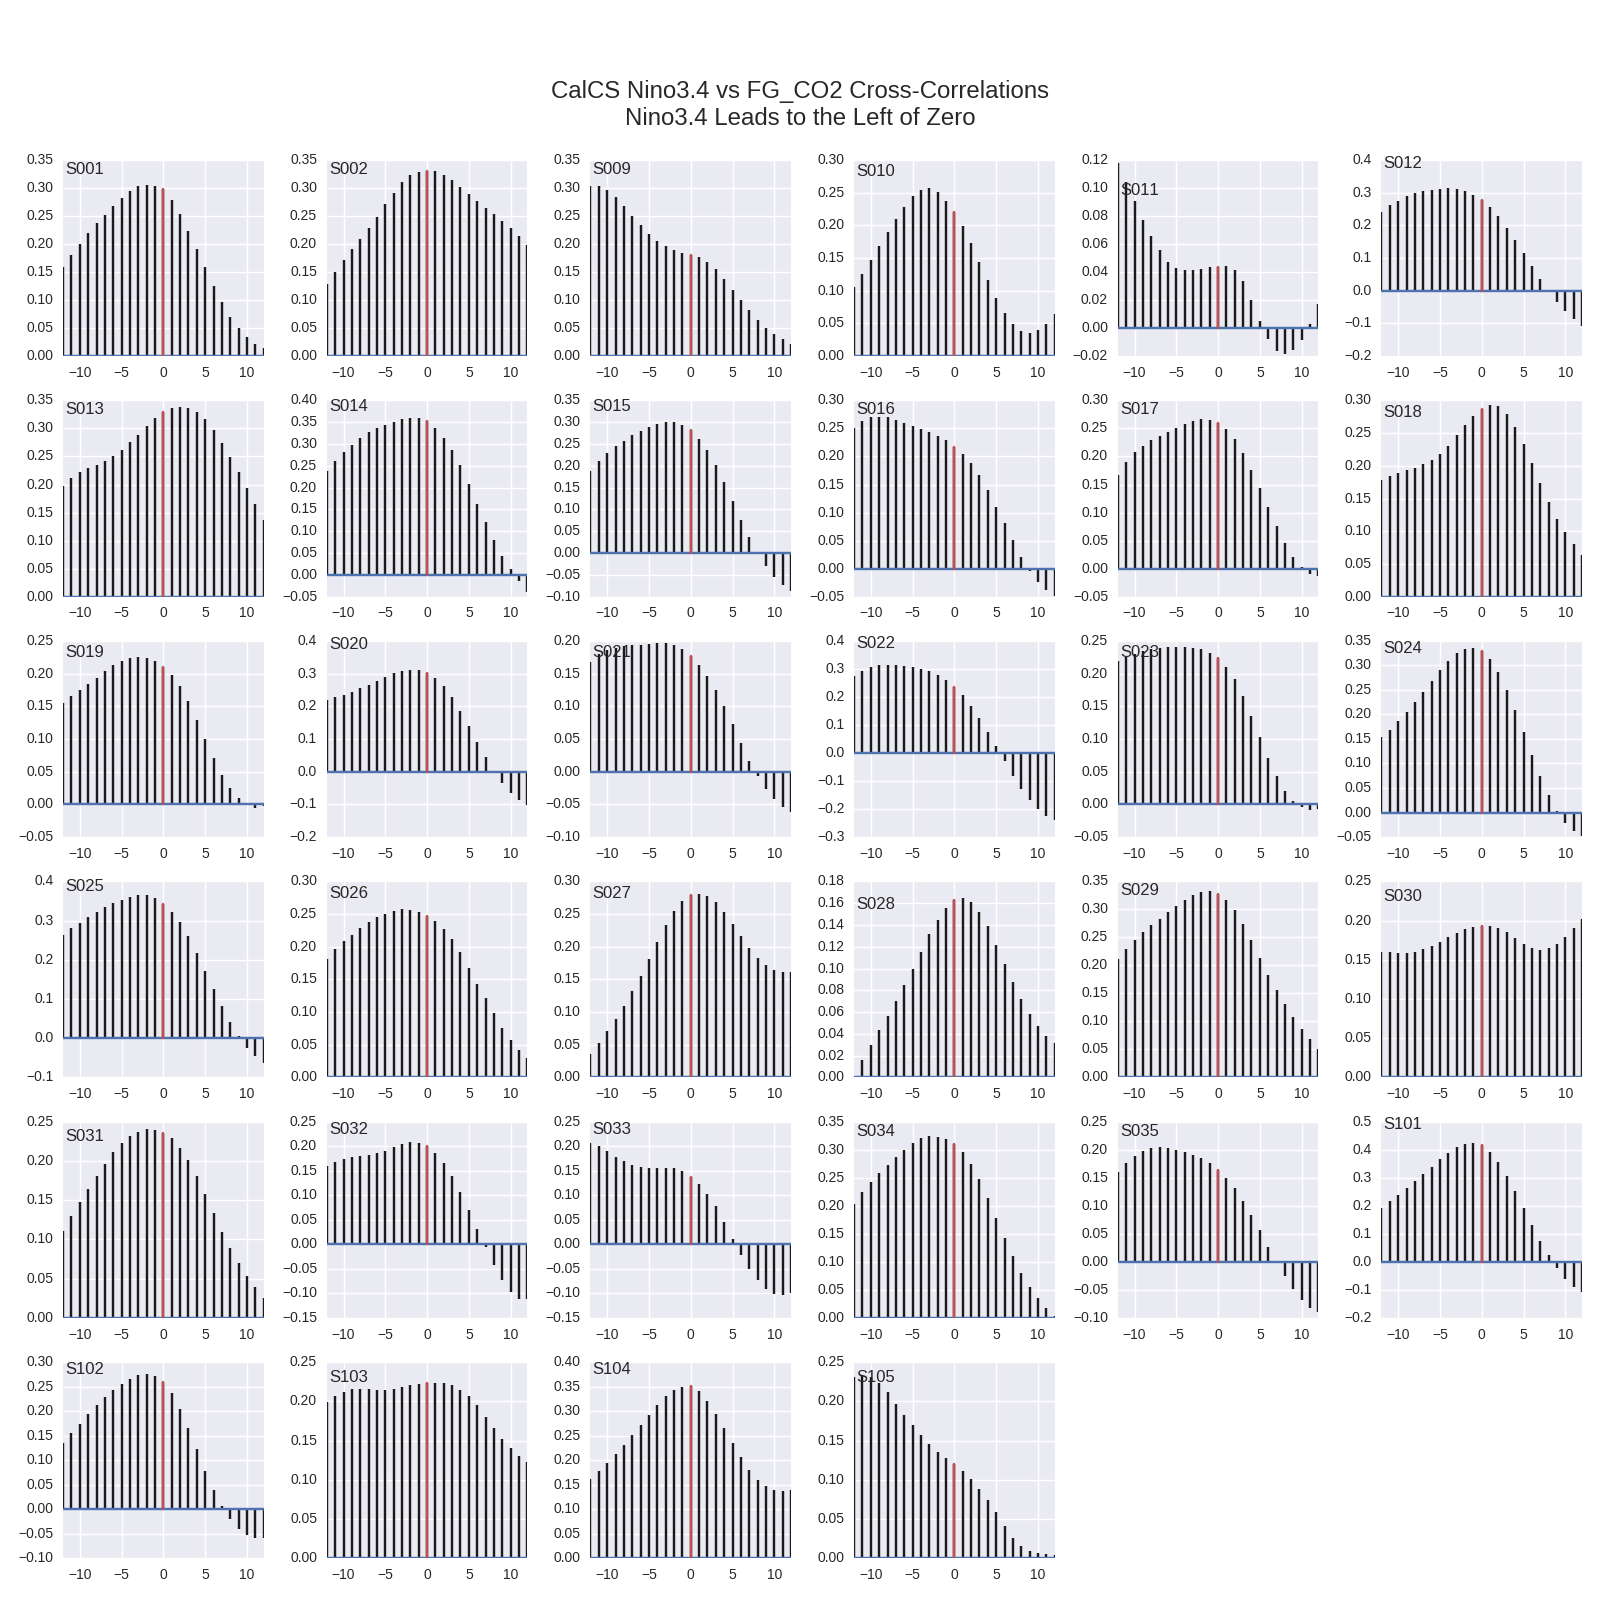
\includegraphics[width=\linewidth]{../../figs/calcs/cross-correlation/Nino34_FGCO2_cross-correlation_CalCS.png}
	\caption{Cross correlations between CalCS FGCO2 and the Nino3.4 index. Negative values indicate ENSO leading FGCO2 in months. The red bar indicates no lag for reference.}
	\label{fig:CalCS-ENSO-Cross}
\end{figure}
\newpage
\begin{figure}[!h]
	\centering
	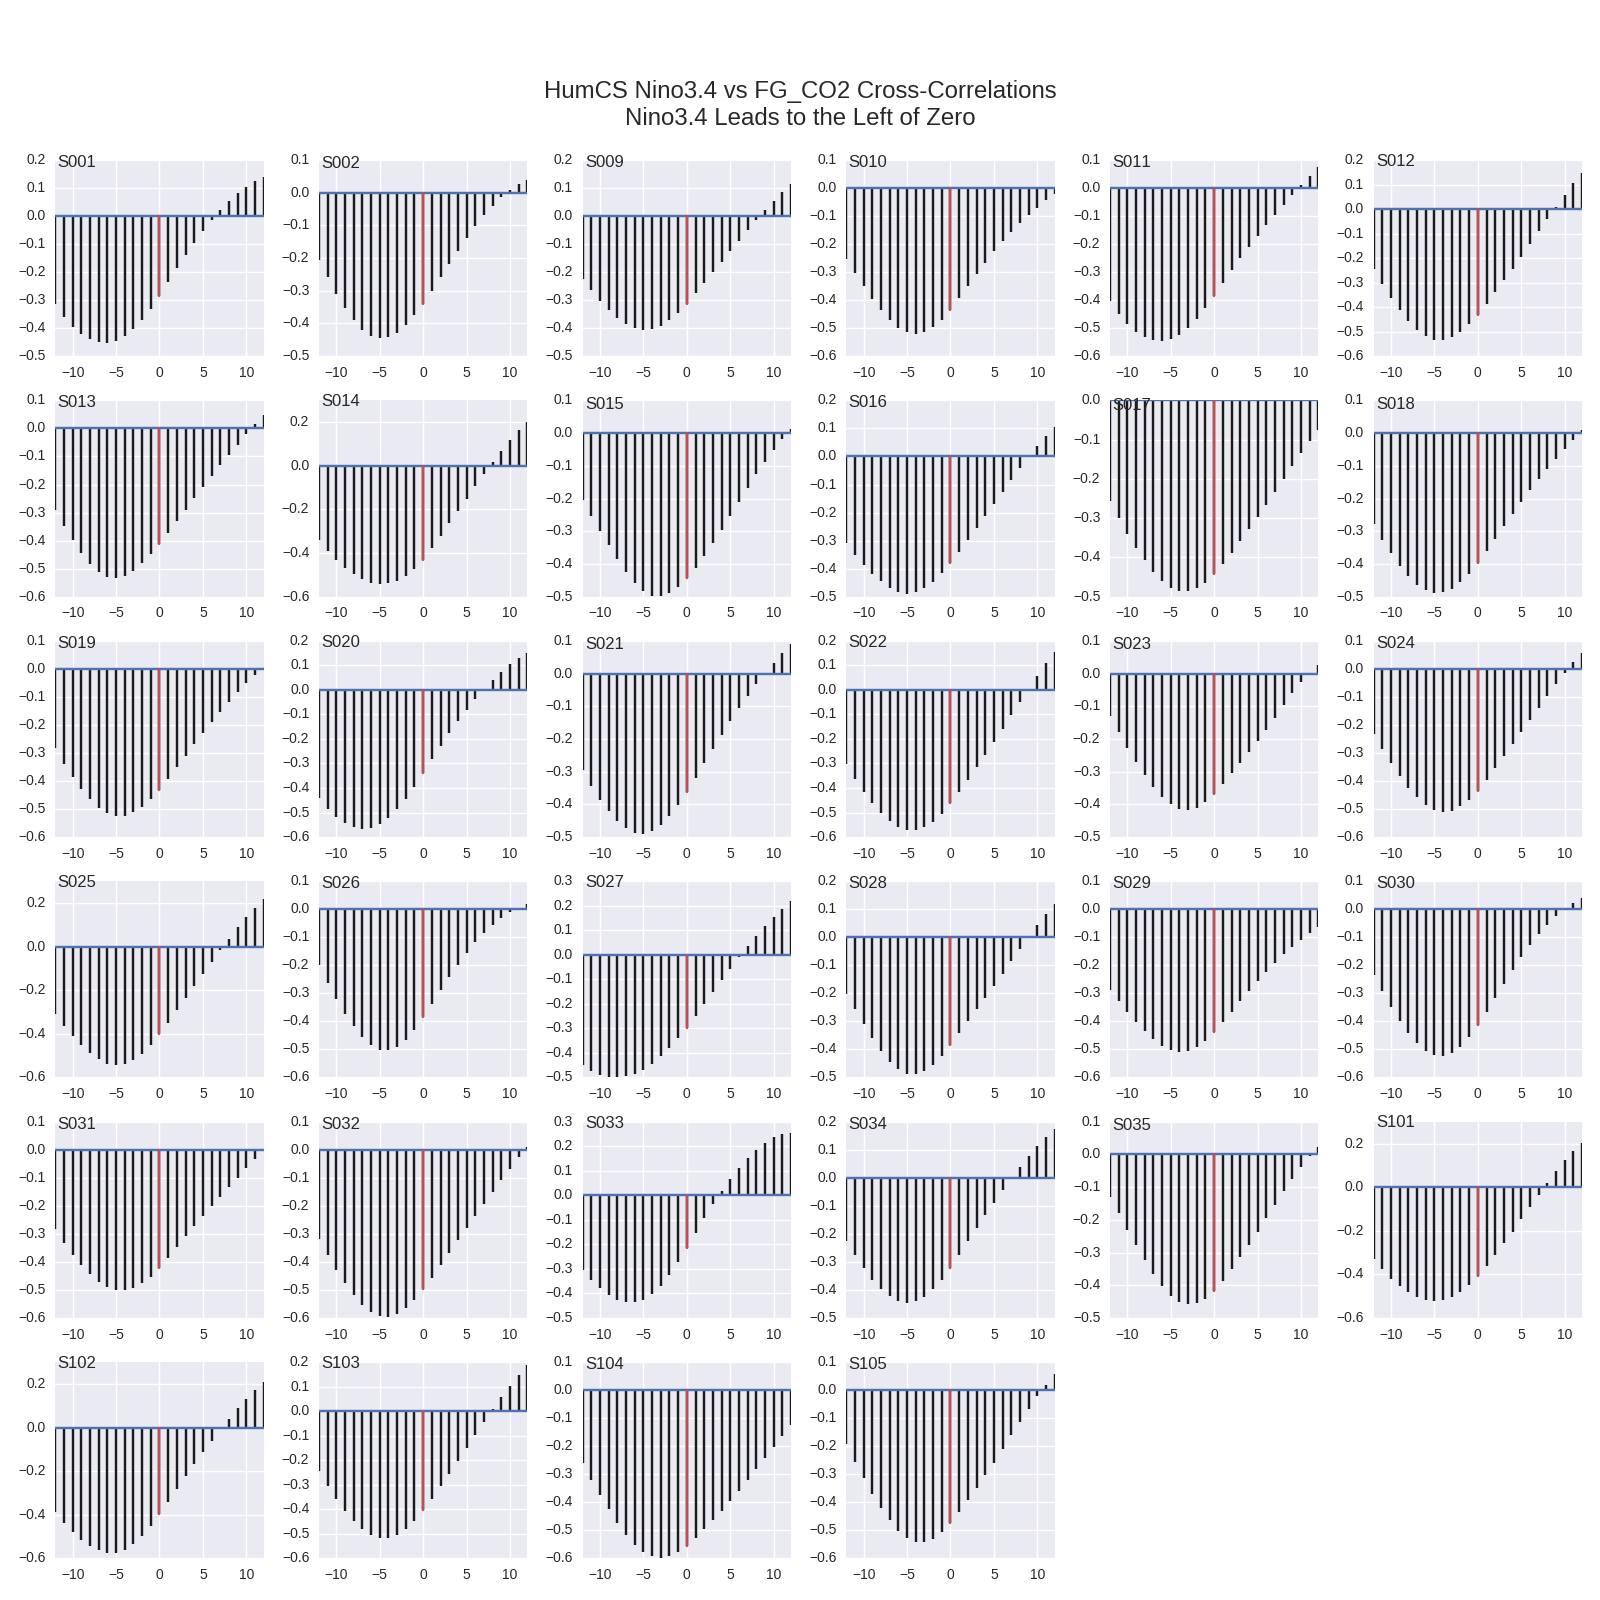
\includegraphics[width=\linewidth]{../../figs/humcs/cross-correlation/Nino34_FGCO2_cross-correlation_HumCS.png}
	\caption{Cross correlations between HumCS FGCO2 and the Nino3.4 index. Negative values indicate ENSO leading FGCO2 in months. The red bar indicates no lag for reference.}
	\label{fig:HumCS-ENSO-Cross}
\end{figure}
\newpage
\begin{figure}[!h]
	\centering
	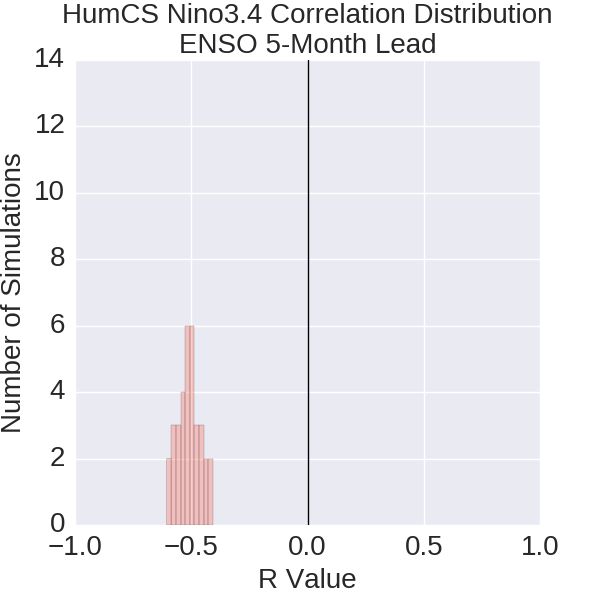
\includegraphics[width=29pc]{../../figs/humcs/histograms/humcs-smoothedFGCO2-enso-lag5-histograms.png}
	\caption{Distribution of r values for a correlation between HumCS FGCO2 anomalies and the Nino3.4 index with a 5-month lead time.}
	\label{fig:HumCS-ENSO-hist-5lag}
\end{figure}

\clearpage
\begin{table}
	\centering
\caption{Results for regressing HumCS FGCO2 anomalies onto Nino3.4 time series with a 5-month lead. Results with $p$ $>$ 0.05 are excluded.}	
\begin{tabular}{c c c c}
	\toprule
	\textbf{Simulation} &  \textbf{Slope}$^{a}$  &  \textbf{R} &  \textbf{R$^{2}$} \\
	\midrule
	0  &  -0.31 &    -0.45 &       0.20 \\
	1  &  -0.41 &    -0.46 &       0.21 \\
	2  &  -0.31 &    -0.41 &       0.17 \\
	3  &  -0.40 &    -0.52 &       0.27 \\
	4  &  -0.40 &    -0.55 &       0.30 \\
	5  &  -0.39 &    -0.54 &       0.29 \\
	6  &  -0.43 &    -0.54 &       0.29 \\
	7  &  -0.38 &    -0.56 &       0.31 \\
	8  &  -0.38 &    -0.49 &       0.24 \\
	9  &  -0.41 &    -0.49 &       0.24 \\
	10 &  -0.28 &    -0.48 &       0.23 \\
	11 &  -0.41 &    -0.49 &       0.24 \\
	12 &  -0.43 &    -0.53 &       0.28 \\
	13 &  -0.35 &    -0.58 &       0.34 \\
	14 &  -0.38 &    -0.49 &       0.24 \\
	15 &  -0.45 &    -0.57 &       0.33 \\
	16 &  -0.34 &    -0.41 &       0.17 \\
	17 &  -0.38 &    -0.51 &       0.26 \\
	18 &  -0.40 &    -0.55 &       0.30 \\
	19 &  -0.41 &    -0.50 &       0.25 \\
	20 &  -0.35 &    -0.47 &       0.22 \\
	21 &  -0.33 &    -0.49 &       0.24 \\
	22 &  -0.45 &    -0.52 &       0.27 \\
	23 &  -0.37 &    -0.52 &       0.27 \\
	24 &  -0.41 &    -0.50 &       0.25 \\
	25 &  -0.46 &    -0.61 &       0.37 \\
	26 &  -0.29 &    -0.43 &       0.19 \\
	27 &  -0.34 &    -0.45 &       0.20 \\
	28 &  -0.32 &    -0.43 &       0.19 \\
	29 &  -0.36 &    -0.53 &       0.28 \\
	30 &  -0.35 &    -0.58 &       0.34 \\
	31 &  -0.37 &    -0.52 &       0.27 \\
	32 &  -0.44 &    -0.59 &       0.34 \\
	33 &  -0.50 &    -0.55 &       0.30 \\
	\bottomrule
	\textbf{Mean} & -0.38 & -0.51 & 0.26  \\
	\textbf{Std} & 0.05 & 0.05 & 0.05  \\
\end{tabular}
\begin{tablenotes}
	\centering
	\item $^{a}$ mol/m$^{2}$/yr/degC
\end{tablenotes}
\label{tab:HumCS-ENSO-5lag}
\end{table}

\clearpage
\section{Spatial Correlation}
The above correlation results are built upon quite large EBUS regions--we generate area-weighted time series over a 1000km meridional and 800km zonal region. What if there are nuances on a finer spatial scale? Perhaps there is some sort of spatial structure, such as an r-value dipole, that we are missing out on. \\

For the CalCS, FGCO2 correlations with ENSO are rather homogeneous (Figure~\ref{fig:CalCS-ENSO-Spatial}). In most simulations, we find a consistent positive correlation throughout the study area--during an El Ni\~no, there is an anomalous CO$_{2}$ outgassing. However, an interesting structure emerges from correlations with PDO (Figure~\ref{fig:CalCS-PDO-Spatial})--the stronger predictor of the two climate indices (Table~\ref{tab:pdo-pacific}). In a majority of simulations, we find a positive relationship with offshore FGCO2 and PDO (a positive PDO event causes anomalous outgassing), but a negative relationship with coastal FGCO2 along California. \\

For the HumCS, I assess the spatial correlation of FGCO2, lead by 5 months by ENSO, due to its stronger relationship (see above sections). In general, we find strong negative correlations throughout the offshore region and coastal south-central Peru (Figure~\ref{fig:HumCS-ENSO5-Spatial}). In some simulations, we find a similar equatorward dipole as between CalCS FGCO2 and PDO. Except, in this case, it is of opposing sign. The spatial correlations between HumCS FGCO2 and PDO shows a clearer emergence of this dipole (Figure~\ref{fig:HumCS-PDO-Spatial}), although the correlations are weaker overall than with ENSO (a point found in Table~\ref{tab:pdo-pacific}). \\

The spatial correlations between CanCS and ENSO resulted in a pretty consistent positive correlation throughout the region, with no meaningful pattern emergence. Plots were not produced for the BenCS, due to its low or insignificant correlation scores with all of the major climate indices.

\newpage
\begin{figure}[!h]
	\centering
	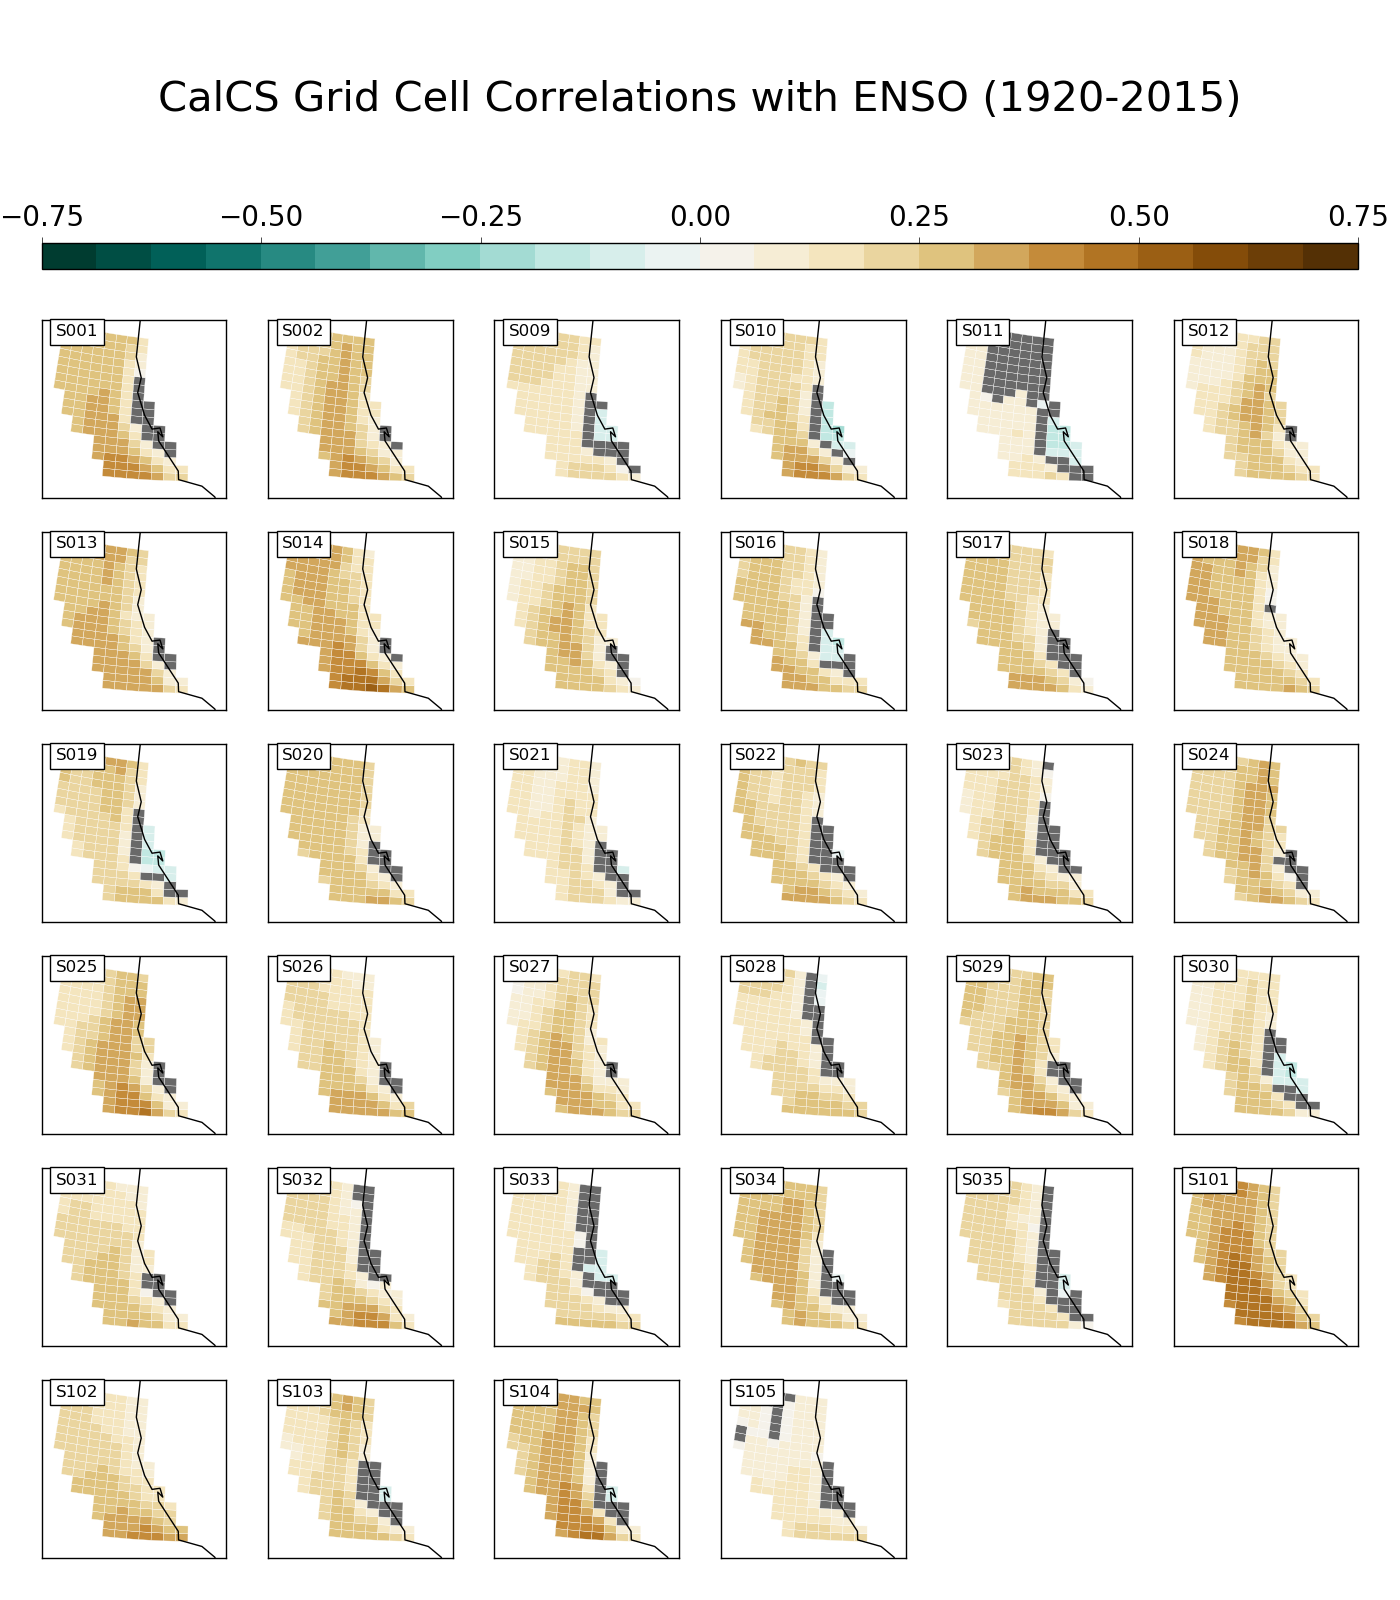
\includegraphics[width=\linewidth]{../../figs/calcs/spatial-correlations/calcs-grid-cell-correlations-nino34-postage.png}
	\caption{Grid cell correlations with the Nino3.4 index in the CalCS. Brown colors are positive r-values, while blue colors are negative r-values. Gray grid cells were analyzed, but have $p$ $>$ 0.05.}
	\label{fig:CalCS-ENSO-Spatial}
\end{figure}
\newpage
\begin{figure}[!h]
	\centering
	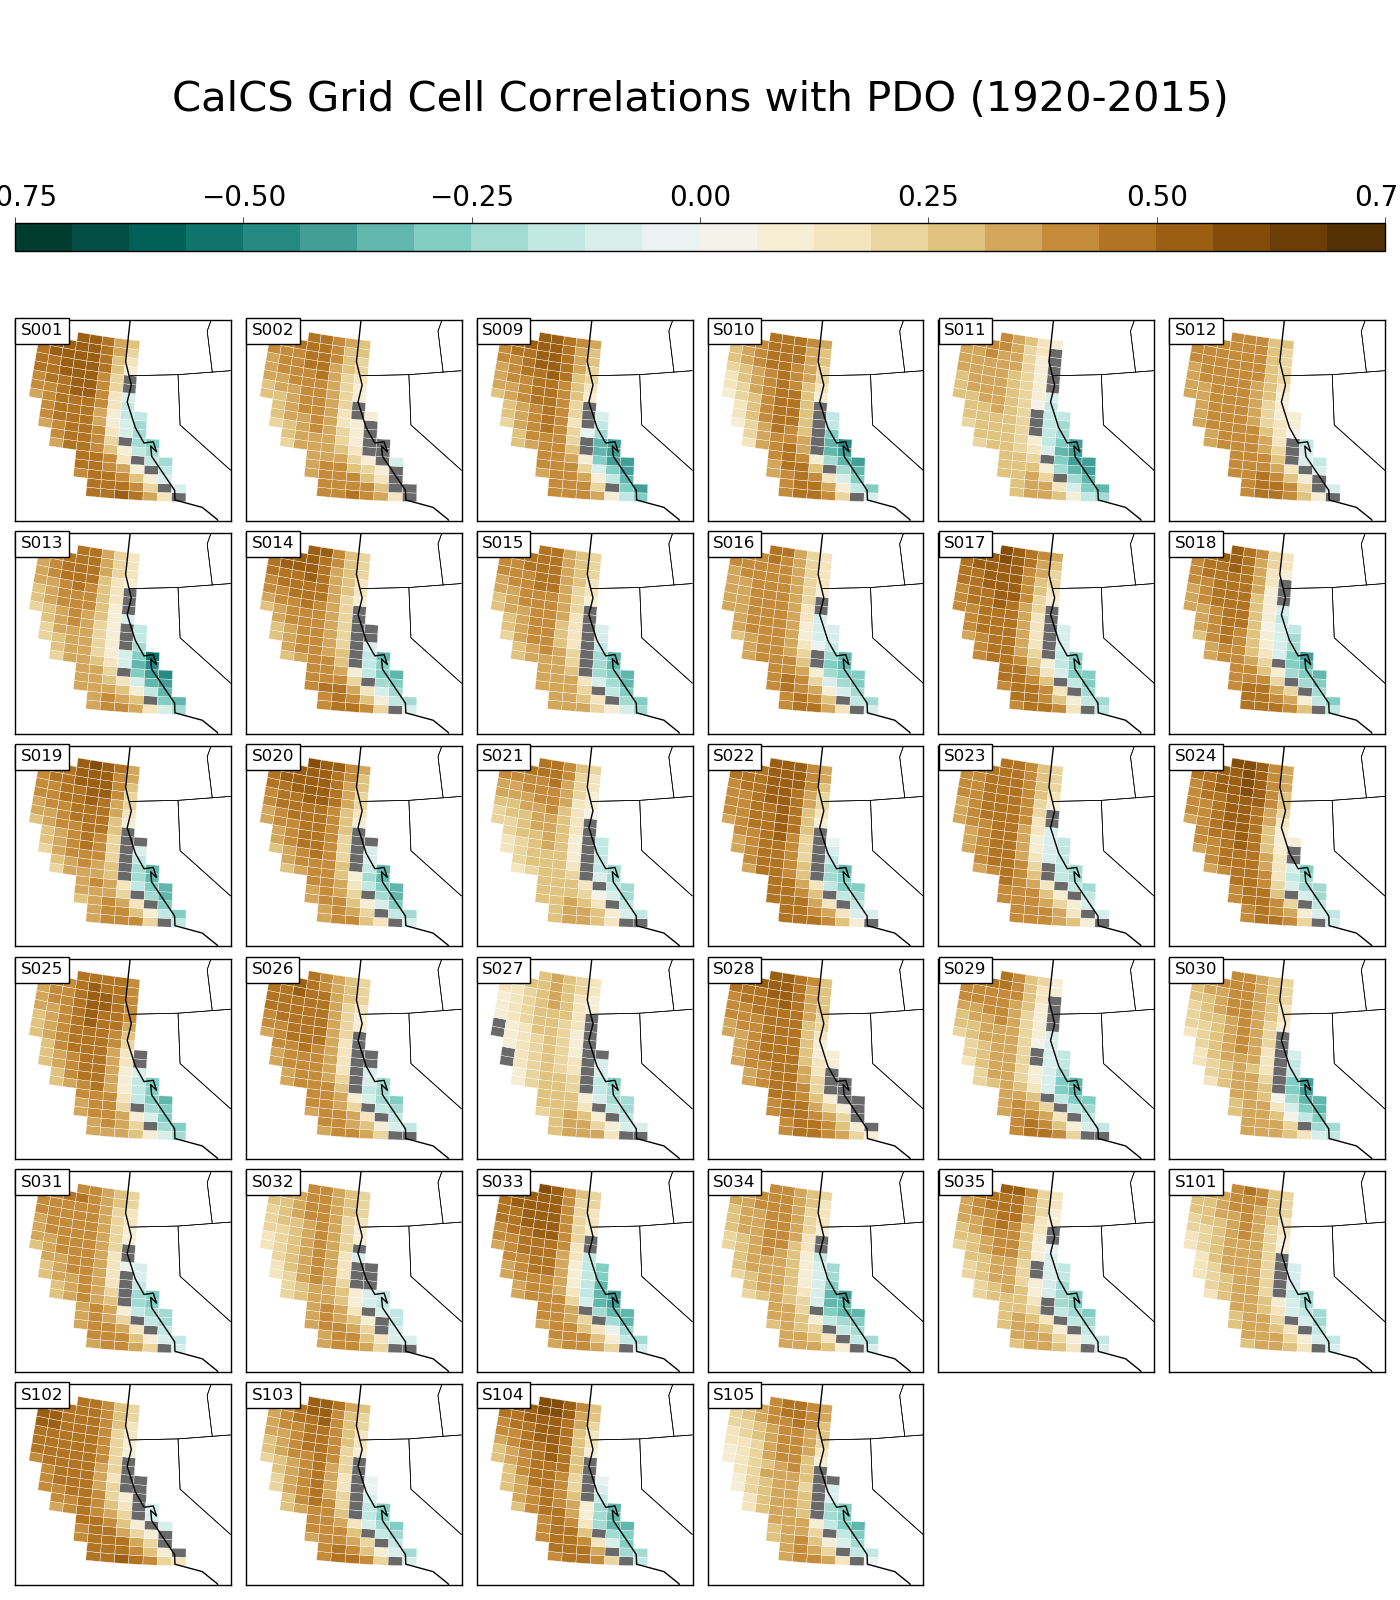
\includegraphics[width=\linewidth]{../../figs/calcs/spatial-correlations/calcs-grid-cell-correlations-pdo-postage.png}
	\caption{Grid cell correlations with PDO index in the CalCS. Brown colors are positive r-values, while blue colors are negative r-values. Gray grid cells were analyzed, but have $p$ $>$ 0.05.}
	\label{fig:CalCS-PDO-Spatial}
\end{figure}
\newpage
\begin{figure}[!h]
	\centering
	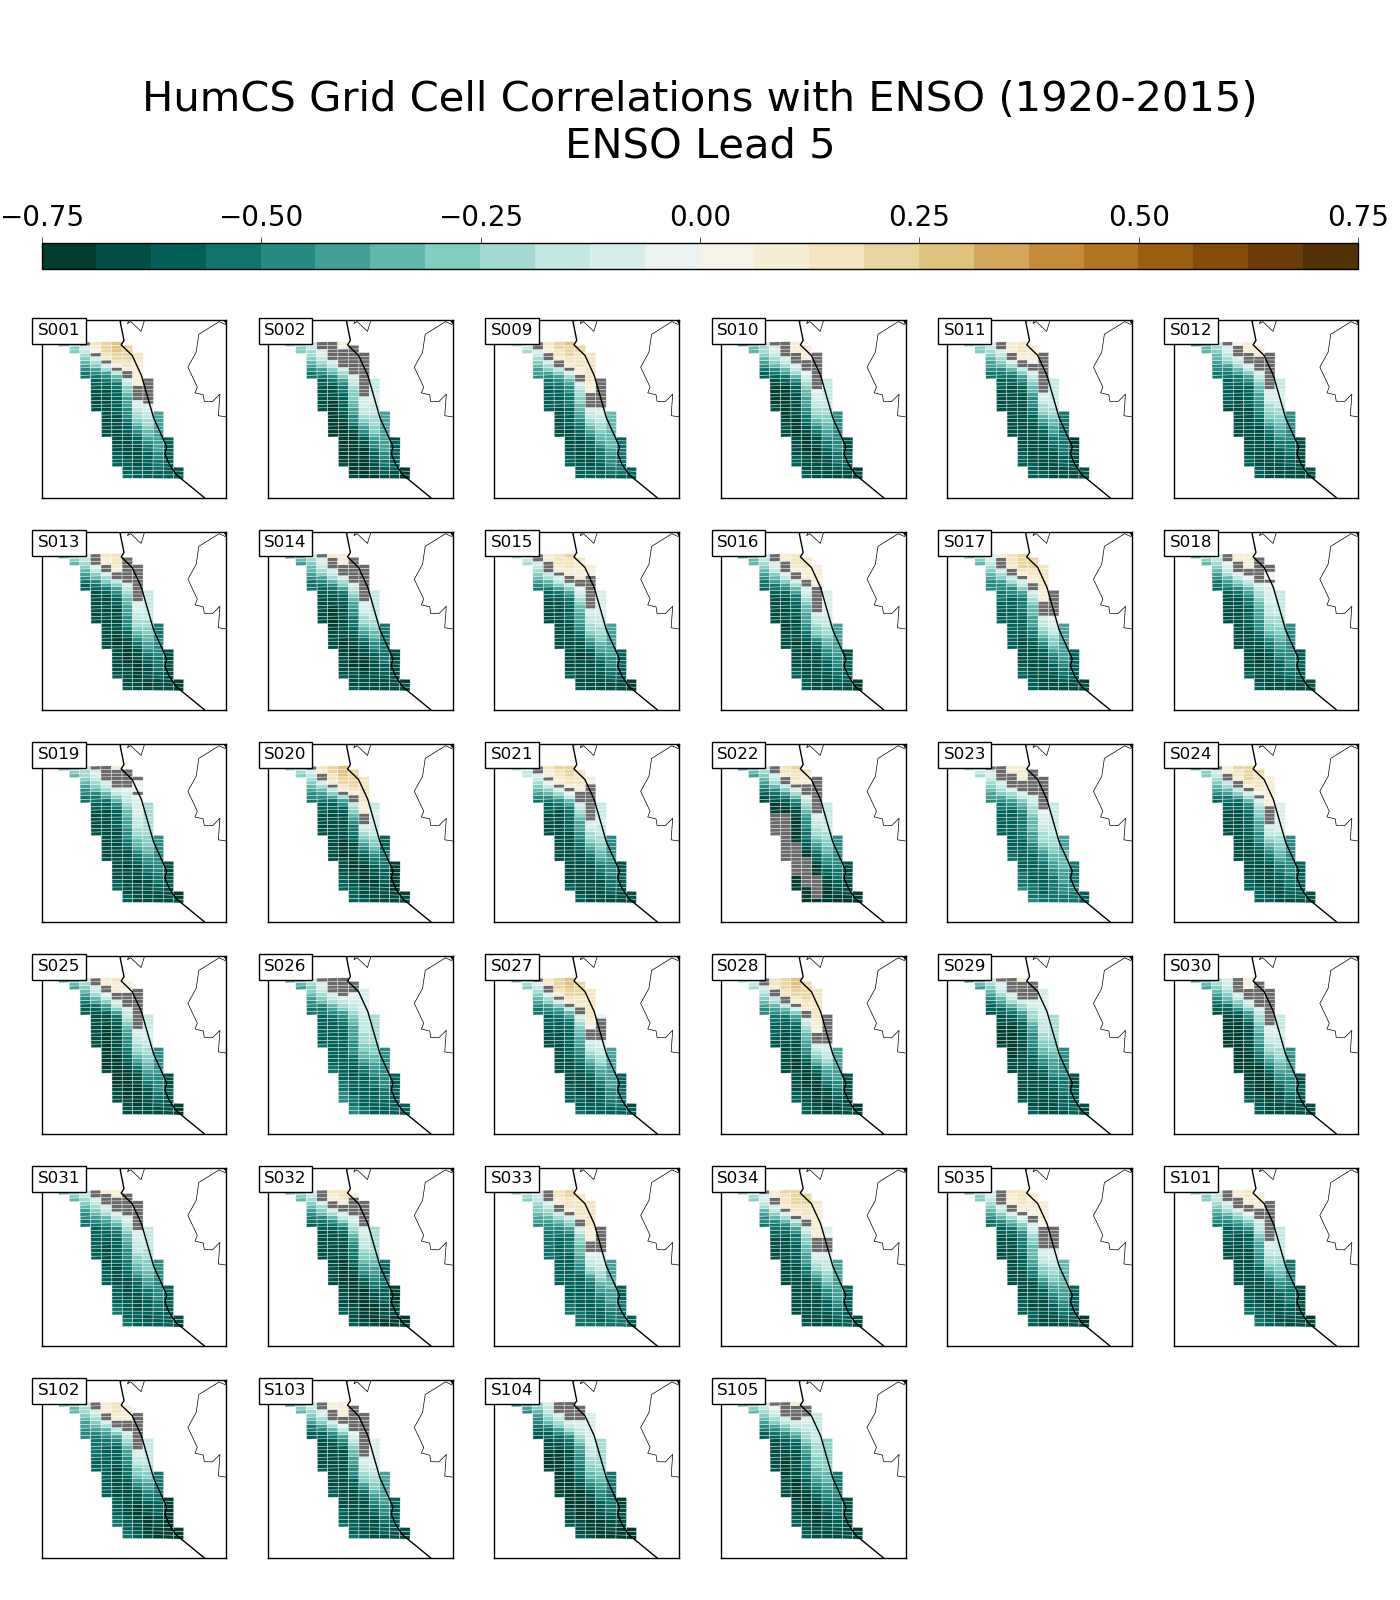
\includegraphics[width=\linewidth]{../../figs/humcs/spatial-correlations/humcs-grid-cell-correlations-nino34-postage-lag5.png}
	\caption{Grid cell correlations with Nino3.4 index (5 month lead) in the HumCS. Brown colors are positive r-values, while blue colors are negative r-values. Gray grid cells were analyzed, but have $p$ $>$ 0.05.}
	\label{fig:HumCS-ENSO5-Spatial}
\end{figure}
\newpage
\begin{figure}[!h]
	\centering
	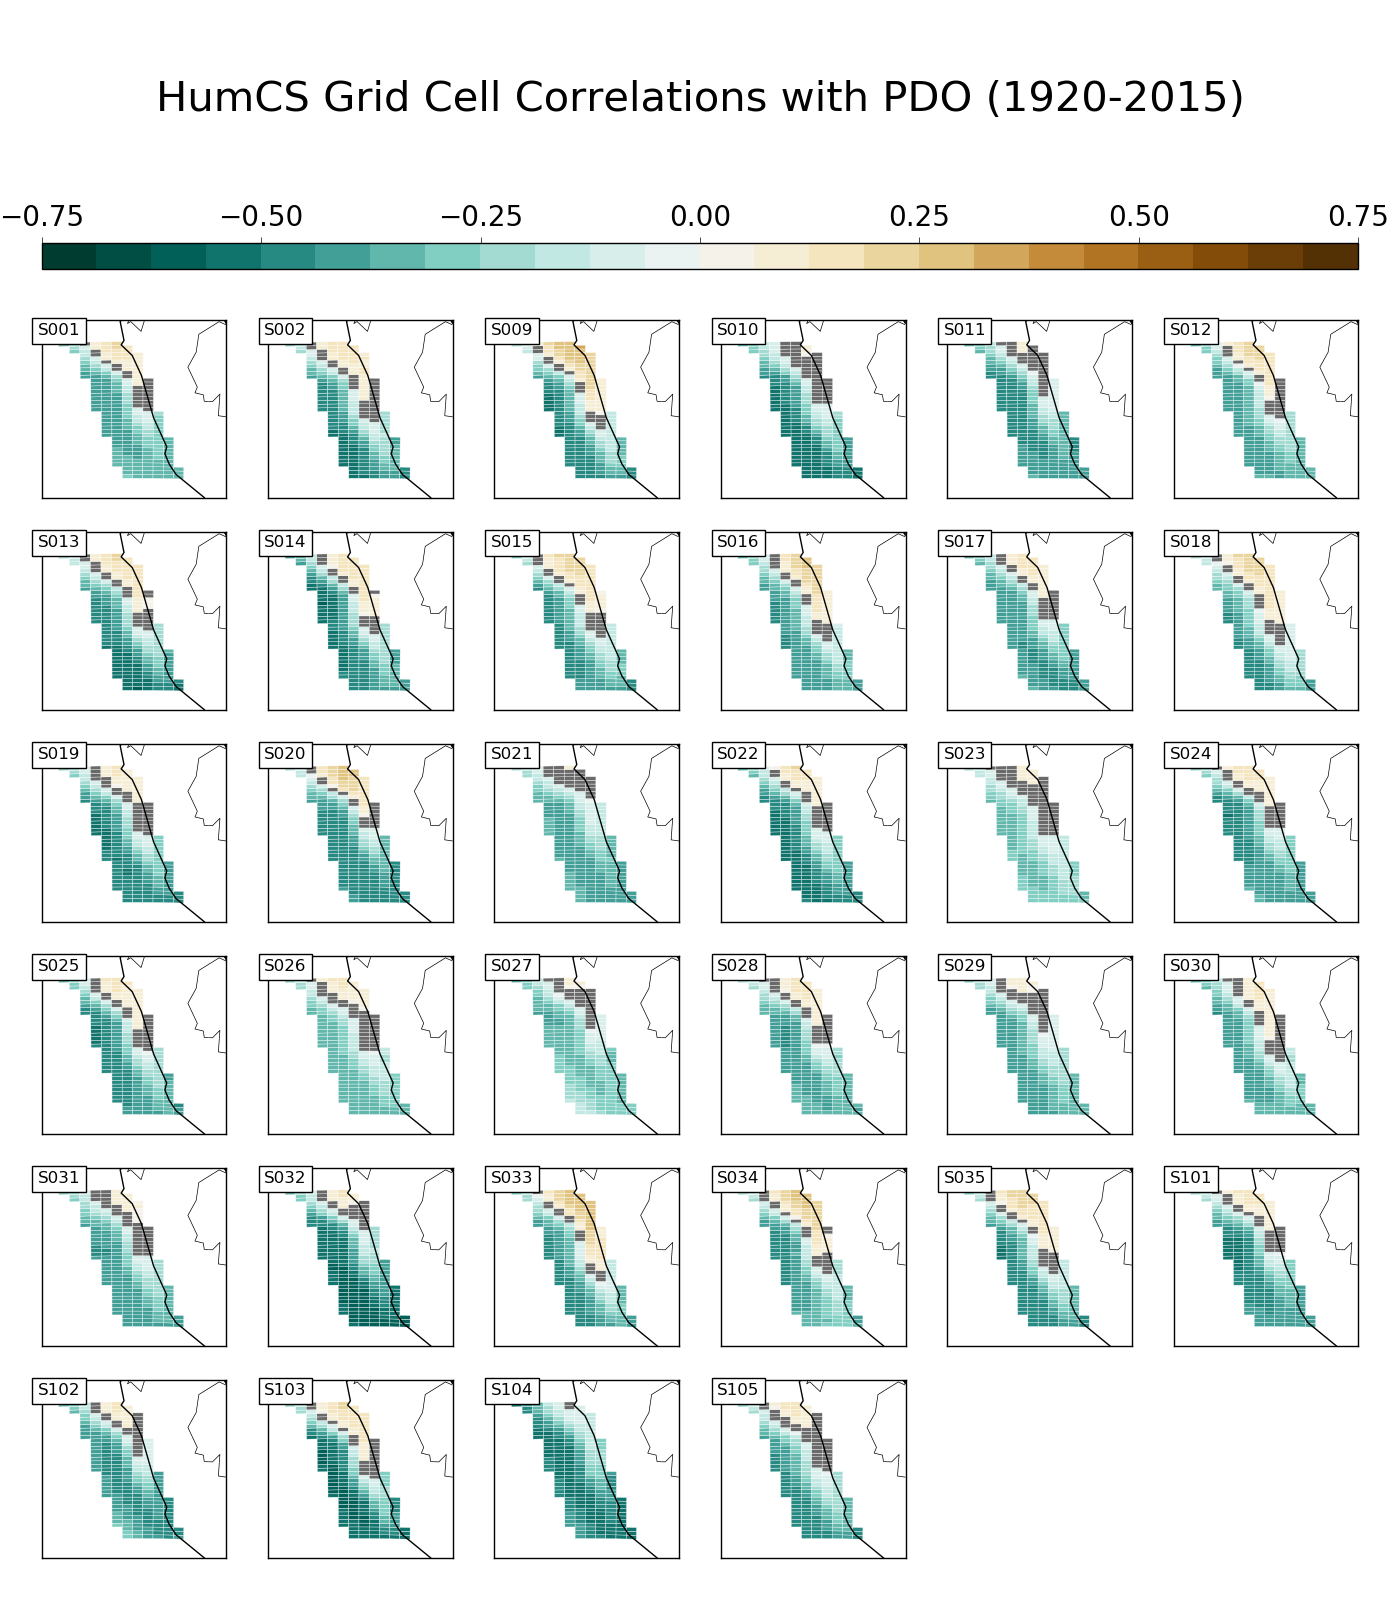
\includegraphics[width=\linewidth]{../../figs/humcs/spatial-correlations/humcs-grid-cell-correlations-pdo-postage.png}
	\caption{Grid cell correlations with the PDO index in the HumCS. Brown colors are positive r-values, while blue colors are negative r-values. Gray grid cells were analyzed, but have $p$ $>$ 0.05.}
	\label{fig:HumCS-PDO-Spatial}
\end{figure}



\clearpage
\bibliography{../../EBUS_BGC_Bibliography.bib}
\end{document}
